%!TEX program = pdflatex
\documentclass[a4paper]{cas-dc}

% ------ packages (only those NOT auto-loaded by cas-dc) ------
\usepackage{amsmath,amssymb}
\usepackage{enumitem}
\usepackage[numbers]{natbib}
\usepackage{colortbl}

\begin{document}
\let\WriteBookmarks\relax
\def\floatpagepagefraction{1}
\def\textpagefraction{.001}

% ------ frontmatter ------
\shorttitle{Multi-Source Heterogeneous Data Fusion for Crypto Return Forecasting}
\shortauthors{M. He}

\title [mode = title]{Multi-Source Heterogeneous Data Fusion for Cryptocurrency Return Forecasting: On the Conditional Effectiveness of On-Chain Indicators}

\author[1]{Minghan He\\[2pt]{\small ORCID: \href{https://orcid.org/0009-0005-7993-6614}{0009-0005-7993-6614}}}
\cormark[1]
\ead{20251513112@sspu.edu.cn}

\affiliation[1]{organization={School of Computer and Information Engineering,
  Shanghai Polytechnic University},
  city={Shanghai},
  postcode={201209},
  country={China}}

\cortext[cor1]{Corresponding author.}

\credit{Conceptualization, Methodology, Software, Validation, Formal analysis, Investigation, Data curation, Writing -- original draft, Writing -- review \& editing, Visualization}

\begin{abstract}
Multi-source heterogeneous data fusion is central to modern financial forecasting, yet a systematic understanding of \textit{when} and \textit{under what conditions} a specific data source contributes incremental predictive value remains lacking. This paper addresses this gap through a large-scale empirical study of on-chain indicators for Bitcoin 4-hour return forecasting, examining how their predictive value depends on companion data sources and model architectures within a unified fusion framework.

We construct six multi-source heterogeneous feature configurations that combine market data, funding rates, sentiment indicators, and both short-term and long-term on-chain metrics, systematically isolating independent contributions from synergistic interactions. Ten models spanning six architectural families---CNN-Transformer, LSTM-Transformer, Transformer, LSTM, TCN, ModernTCN, PatchTST, DLinear, TimeMixer, and XGBoost---are evaluated under this fusion framework with multi-seed evaluation, sliding-window validation, transaction-cost analysis, and statistical significance testing.

Results reveal that short-term on-chain indicators alone offer negligible predictive value---no model achieves a positive test Sharpe when on-chain data is paired only with price features. When fused with funding-rate and sentiment features, however, substantial nonlinear synergy emerges, but this synergy is strongly architecture-dependent. The ten models separate cleanly into three groups: a synergistic-utilization group (CNN-Transformer, LSTM-Transformer; $\Delta$Sharpe $>+2$), a neutral group (Transformer, PatchTST, DLinear, XGBoost; $\Delta$Sharpe $\approx 0$), and a negative-interference group (LSTM, TCN, ModernTCN, TimeMixer; $\Delta$Sharpe $<-1.5$). TimeMixer (ICLR 2024) achieves the highest Sharpe (4.89) on price\_funding\_fng yet collapses when on-chain features are added ($\Delta$Sharpe $-3.11$), providing the strongest counterexample. This three-group architecture pattern is robust across five random seeds and eight sliding-window market regimes. Hybrid architectures also demonstrate superior cost resilience (break-even $\sim$47 bps vs.\ $\sim$27 bps for pure architectures), behaviorally rooted in moderate turnover rates.

We distill these findings into a conditional-effectiveness principle for heterogeneous data fusion: a data source's predictive value is not intrinsic but depends on the three-way alignment among indicator type, companion modalities, and model architecture. This principle, together with the three-group architecture taxonomy and the multi-dimensional evaluation framework we establish, constitutes the paper's core contribution and carries direct implications for feature engineering and model selection in multi-source financial forecasting systems.
\end{abstract}

\begin{highlights}
\item Multi-source heterogeneous data fusion framework integrating market data, funding rates, sentiment indicators, and on-chain metrics for cryptocurrency return forecasting.
\item Discovery of conditional effectiveness: on-chain indicators (SOPR/CDD) provide no independent predictive power, yet produce statistically significant Sharpe gains ($\Delta$Sharpe $>+2$, $p<0.05$) when fused with funding rate and sentiment data---but only under architectures capable of cross-source interaction.
\item Three-group architecture taxonomy for heterogeneous data fusion: across ten models spanning six families, architectures divide into synergistic-utilization (CNN/LSTM-Transformer), neutral (Transformer, PatchTST, DLinear, XGBoost), and negative-interference groups (LSTM, TCN, ModernTCN, TimeMixer). TimeMixer (ICLR 2024) achieves Sharpe 4.89 on price+funding+sentiment yet collapses to 1.78 when on-chain features are fused ($\Delta$Sharpe $-$3.11).
\item Hybrid architectures exhibit approximately double the cost resilience of pure architectures (break-even $\sim$47 bps vs.\ $\sim$27 bps), and the three-group taxonomy remains robust across eight market regimes (2022--2025). XGBoost's static Sharpe (4.50) collapses under temporal cross-validation (mean $-$0.79), demonstrating that single-window evaluation can mislead model selection in financial forecasting.
\end{highlights}

\begin{keywords}
multi-source data fusion \sep cryptocurrency \sep return forecasting \sep on-chain data \sep heterogeneous data \sep deep learning \sep conditional effectiveness
\end{keywords}

\maketitle

\setlength{\emergencystretch}{1em}

% ================================================================
%  1. Introduction
% ================================================================
\section{Introduction}

The proliferation of heterogeneous data sources in finance---market prices, derivative signals, sentiment indicators, and blockchain-derived on-chain metrics---has created both opportunities and challenges for predictive modeling. While multi-source data fusion is widely practiced, a fundamental question remains: \textit{how can one systematically determine whether, and under what conditions, fusing a specific data source yields incremental predictive value?} Existing work largely adopts an ad-hoc approach, either stacking all available sources without isolating individual contributions, or testing sources in isolation which overlooks nonlinear synergistic interactions. A principled framework for evaluating fusion effectiveness across data modalities and model architectures is lacking.

Cryptocurrency markets, with their rich ecosystem of heterogeneous data streams, offer an ideal test bed for studying this question~\cite{urquhart2016,kristoufek2015}. On-chain data---including short-term holder behavior metrics (SOPR/CDD) and long-term supply-demand metrics (exchange balances, active addresses, netflow)---has been widely regarded as a valuable yet poorly understood information source. Prior work either incorporates on-chain data as auxiliary features without systematic evaluation, or analyzes its long-term relationship with prices at low frequencies, leaving its incremental fusion value at short horizons unresolved.

This paper addresses these gaps through a systematic multi-source fusion study. We design six heterogeneous feature configurations on Bitcoin 4-hour candlestick data that operationally isolate the independent versus synergistic contributions of on-chain data, and conduct a fair comparison across ten representative models spanning six architectural families. The main contributions are as follows:

\begin{enumerate}[label=(\arabic*),leftmargin=1.5em]
    \item Discovery of conditional effectiveness. Through systematic feature ablation, we establish that on-chain data's predictive value is conditional rather than universal: short-term on-chain indicators (SOPR/CDD) offer no independent predictive power, yet produce large and statistically significant $\Delta$Sharpe gains once funding-rate and sentiment features are present (robust across five random seeds, $p<0.05$ in DM tests); long-term on-chain indicators (exchange balances, active addresses, netflow) exhibit no predictive value at the 4-hour frequency and may introduce noise.
    \item Three-group architecture taxonomy. Cross-model comparison reveals a clear architecture-dependent pattern in exploiting on-chain synergy---the ten models separate into three groups based on their $\Delta$Sharpe from price\_funding\_fng to full: synergistic-utilization (CNN-Transformer, LSTM-Transformer; $\Delta$Sharpe $> +2$), neutral (Transformer, PatchTST, DLinear, XGBoost; $\Delta$Sharpe $\approx 0$), and negative-interference (LSTM, TCN, ModernTCN, TimeMixer; $\Delta$Sharpe $< -1.5$). TimeMixer (ICLR 2024) achieves the highest Sharpe on price\_funding\_fng (4.89) yet collapses when on-chain features are added ($\Delta$Sharpe $-3.11$), providing the strongest counterexample to the architecture-dependence thesis. DLinear and TimeMixer falling into the neutral and negative-interference groups respectively confirms the completeness of this taxonomy from both the minimalist and cutting-edge ends of the architectural spectrum.
    \item Multi-dimensional evaluation framework and deployment insights. We construct an evaluation framework spanning prediction accuracy to deployment feasibility (Rank IC, Sharpe ratio, maximum drawdown, Diebold--Mariano and Bootstrap tests, cost sensitivity, and turnover analysis). Sliding-window validation across eight market regimes (2022--2025) confirms the temporal robustness of the three-group architecture pattern---the synergistic-utilization group achieves the highest cross-window mean Sharpe (3.85). We further discover that hybrid architectures exhibit approximately double the cost resilience of pure architectures (break-even $\sim$47 bps vs.\ $\sim$27 bps), and that XGBoost's high static Sharpe (4.50) disappears entirely under temporal cross-validation (mean $-0.79$)---a methodological caution for financial forecasting evaluation.
\end{enumerate}

\section{Related Work}

\subsection{Cryptocurrency Return Prediction}

Traditional methods such as ARIMA and GARCH have well-known limitations in the high-volatility setting of cryptocurrencies~\cite{catania2019,kristoufek2015}. XGBoost \cite{chen2016} requires flattening the temporal dimension, losing dependency information. LSTM \cite{hochreiter1997} has been widely applied to financial forecasting \cite{mcnally2018}. The Transformer family, surveyed comprehensively by Wen et al.~\cite{wen2023}, includes architectures such as the Temporal Fusion Transformer~\cite{lim2021}, PatchTST \cite{nie2023}, and ModernTCN \cite{luo2024}. Additionally, DLinear \cite{zeng2023} demonstrated that simple channel-independent linear decomposition can be surprisingly competitive in long-sequence forecasting, raising fundamental questions about the necessity of complex architectures. TimeMixer \cite{wang2024timemixer} further advanced the field with a multi-scale decomposable mixing framework (PDM+FMM), achieving state-of-the-art results at ICLR 2024. Both are included in our comparison to span the full architectural spectrum from ``minimalist linear'' to ``multi-scale mixing.''

\subsection{Multi-Source Data Fusion and On-Chain Data Analysis}

The funding rate reflects periodic payments between long and short traders in perpetual contracts~\cite{malik2023}, and the Fear \& Greed Index aggregates volume, volatility, and social media sentiment to quantify market psychology~\cite{carosia2024}. On-chain data reveals supply-demand dynamics: SOPR (Spent Output Profit Ratio) measures the weighted average profit/loss of on-chain moved BTC, and CDD (Coin Days Destroyed) weights transactions by holding duration to identify long-term holder activity. These short-term indicators have been used for market cycle turning point identification, yet their predictive value at the 4-hour level remains untested. Long-term indicators (exchange balances, active addresses, netflow) reflect macro-level supply-demand trends with longer fluctuation cycles and may suffer from a granularity mismatch with the 4-hour frequency. Early works~\cite{alessandretti2018} demonstrated the potential of blockchain-derived features for cryptocurrency price prediction, but did not systematically distinguish between short-term and long-term on-chain indicators. More recently, Das et al.~\cite{das2026} combined transformer-based language models with graph neural networks and social media sentiment to predict BTC and ETH prices, further validating the value of sentiment signals in multi-source cryptocurrency forecasting frameworks, although their LSTM-GNN hybrid architecture does not incorporate on-chain data.

Existing research~\cite{corbet2019} has three shortcomings: it does not distinguish short-term from long-term on-chain indicators in terms of predictive granularity; it tests only independent predictive power, overlooking nonlinear synergistic effects; and it lacks systematic investigation of how architectures differ in exploiting on-chain signals. Kim et al.\ (2022)~\cite{kim2022} employed a SAM-LSTM (Self-Attention-based Multiple LSTM) model with on-chain data and change point detection to predict BTC prices, validating the predictive potential of on-chain features. However, their study did not design feature ablation experiments to disentangle the independent versus synergistic contributions of on-chain data, nor did it compare how different architectures exploit on-chain signals.

\subsection{Quantitative Comparison with Existing Work}

Table~\ref{tab:lit_comparison} summarizes the core metrics of representative studies in recent years alongside our results for comparison.

\begin{table*}[t]
\centering
\caption{Core metric comparison of representative cryptocurrency return prediction studies}
\label{tab:lit_comparison}
\footnotesize
\begin{tabular}{lcccc}
\toprule
Study & Model & Directional Acc. & Sharpe & Other Metrics \\
\midrule
Omole \& Enke \cite{omole2024} & CNN-LSTM + Boruta & 82.4\% & 6.47 & Ann.\ return 1682\% \\
Kozhevnikov \cite{kozh2025} & XGBoost (full cycle) & -- & 1.68 & MaxDD $-17.3\%$ \\
Kozhevnikov \cite{kozh2025} & LSTM & 52.4\% & -- & -- \\
Kim et al.\ \cite{kim2022} & SAM-LSTM & -- & -- & On-chain + CPD \\
Hasanli \& Dursun \cite{findev2025} & XGBoost (BTC) & 55.9\% & 1.78 & Cum.\ return 141.4\% \\
Pambudi et al.\ \cite{pambudi2025} & Transformer & -- & -- & MAPE 0.20\% \\
\textbf{This paper} & \textbf{CNN-Transformer} & \textbf{54.7\%} & \textbf{5.19} & \textbf{IC=0.150} \\
\bottomrule
\multicolumn{5}{p{0.85\textwidth}}{\footnotesize Notes: (1) Data periods, frequencies, and cost assumptions differ across studies---the above numbers are not directly comparable; (2) Omole \& Enke use daily data spanning 2012--2023 covering full bull-bear cycles; this paper uses 4-hour frequency; (3) IC (Information Coefficient) is rarely reported in cryptocurrency literature; this paper introduces it as a supplementary metric.}
\end{tabular}
\end{table*}

As shown in Table~\ref{tab:lit_comparison}, the directional accuracy of our CNN-Transformer (54.7\%) shows a modest improvement over the typical LSTM value in the literature (52.4\%). However, data periods, frequencies, and cost assumptions differ across studies, and Sharpe ratios at different frequencies are not directly comparable---annualized Sharpe ratios for high-frequency strategies are naturally inflated by larger sample sizes. Collectively, existing work still lacks a fair comparison between hybrid and pure architectures under a unified framework; feature ablation of on-chain data is mostly validated via ``stacking'' without distinguishing synergistic effects from architectural dependence; and evaluation remains largely at the MSE level, with IC virtually unused.

\section{Data and Feature Engineering}

\subsection{Data Sources and Preprocessing}

This study uses data from the following sources:

\begin{itemize}[leftmargin=1.5em]
    \item Price and volume data: BTC/USDT perpetual contract 1-hour candlestick data from Binance (resampled to 4 hours), including open, high, low, close, and volume.
    \item Funding rate: Perpetual contract funding rate data for the corresponding time windows.
    \item Fear \& Greed Index: Daily data from Alternative.me reflecting market sentiment, forward-filled to 4-hour frequency.
    \item On-chain indicators: From Dune Analytics and OKLink, including SOPR (Spent Output Profit Ratio), CDD (Coin Days Destroyed), total BTC on exchanges, active addresses, and BTC netflow.
\end{itemize}

All data are aligned by timestamp and merged into a unified 4-hour frequency dataset, with missing values handled via forward filling. The final dataset covers January 1, 2020 to May 7, 2026 (4-hour frequency, 13,909 raw records). It is chronologically partitioned into a training set (January 2020--June 2024, 9,736 records, 70\%), a validation set (June 2024--June 2025, 2,086 records, 15\%), and a test set (June 2025--May 2026, 2,087 records, 15\%). After constructing sequences with a lookback window $L=48$, the actual sample counts are 9,702 training, 2,079 validation, and 2,080 test sequences.

\subsection{Feature Construction}

\subsubsection{Price-Based Features}

For each lag step $l \in \{1,2,3,4,6,8,12\}$, the log-return is computed as:
\begin{equation}
\text{ret}_l = \ln \frac{\text{close}_t}{\text{close}_{t-l}}
\end{equation}

Additional features include return acceleration (differences between returns at two different lags), log volume and its rate of change, and price position indicators (HH, LL, and price position ratio) computed from high and low prices.

\subsubsection{Multi-Scale Statistical Features}

For each continuous factor, over windows $w \in \{4,8,12,24\}$, the following are computed:
\begin{equation}
z_w = \frac{x_t - \mu_w}{\sigma_w + \epsilon}
\end{equation}
\begin{equation}
\text{mom}_w = \frac{x_t}{x_{t-w}} - 1
\end{equation}
representing the standardized deviation and window momentum, respectively.

\subsubsection{On-Chain Feature Construction and Selection Rationale}

SOPR and CDD serve as representative short-term on-chain indicators, each yielding 11-dimensional features (raw/log-transformed, first- and second-order differences, 4-window z-scores and momentum, totaling 22 dimensions). Exchange BTC balances, active addresses, and netflow serve as long-term on-chain representatives with fluctuation cycles measured in days or weeks; they are included in the price\_long\_onchain feature set to test their short-term predictive value and are excluded from the full feature set (preliminary experiments confirmed no benefit).

\subsubsection{Cross-Source Interaction Features}

Four types of multiplicative interaction terms are constructed to capture nonlinear coupling between data sources: sentiment--profit/loss (fng\_sopr\_int), whale anomaly--volume (cdd\_vol\_int), funding rate--volatility (fr\_vol\_int), and extreme sentiment--momentum (fng\_mom\_int). The first two depend on SOPR/CDD data and exist only in the full set. Consequently, of the 24-dimensional increment from price\_funding\_fng to full, 22 dimensions are raw on-chain features and 2 are newly added on-chain-dependent interaction terms. Raw on-chain features grant the model greater flexibility in cross-source combination than fixed product terms alone (detailed in Section~6.2).

\subsection{Feature Set Design (Ablation Study)}

To systematically evaluate the contribution of different data sources to prediction---particularly the independent versus synergistic value of on-chain data---six feature configurations are designed, as shown in Table~\ref{tab:feature_sets}. These six configurations are not merely incremental additions but serve three progressive analytical objectives: (1) establishing a pure price baseline via price\_only; (2) testing the independent predictive power of on-chain data when ``only accompanied by price'' via price\_onchain and price\_long\_onchain; (3) testing the incremental synergistic effect of on-chain data when ``derivative and sentiment data are already present'' via the contrast between price\_funding\_fng and full. If full significantly outperforms price\_funding\_fng while price\_onchain performs poorly, this indicates that the value of on-chain data is not independent but conditional---dependent on interaction with other data sources.

\begin{table*}[t]
\centering
\caption{Six feature configurations and their data sources}
\label{tab:feature_sets}
\footnotesize
\begin{tabular}{lcccc}
\toprule
\multirow{2}{*}{Feature Set} & \multicolumn{4}{c}{Data Source} \\
\cmidrule(lr){2-5}
& Price & Funding Rate & Fear \& Greed & On-Chain \\
\midrule
price\_only        & \checkmark & & & \\
price\_funding     & \checkmark & \checkmark & & \\
price\_funding\_fng & \checkmark & \checkmark & \checkmark & \\
price\_onchain     & \checkmark & & & \checkmark \\
price\_long\_onchain & \checkmark & & & \checkmark* \\
full               & \checkmark & \checkmark & \checkmark & \checkmark \\
\bottomrule
\multicolumn{5}{p{0.85\textwidth}}{\footnotesize *Only price\_long\_onchain includes long-term on-chain indicators (exchange balances, active addresses, netflow); the on-chain features in full are SOPR and CDD; long-term indicators were excluded due to poor performance in tests.}
\end{tabular}
\end{table*}

Sequence construction uses a sliding window approach with a lookback window $L=48$ (48 past 4-hour candles, approximately 8 days) and a prediction horizon $H=1$ (next 4-hour log-return). Feature set dimensionalities are: price\_only 18, price\_funding 28, price\_funding\_fng 40, price\_onchain 40, price\_long\_onchain 48, full 64.

The dataset is chronologically split into training (first 70\%), validation (middle 15\%), and test (last 15\%) sets. Feature standardization employs RobustScaler (5\%--95\% quantile range) to mitigate the influence of extreme values on deep learning training. The scaler is fitted only on the training set (fit\_transform) with validation and test sets receiving transform only, preventing future information leakage.

\subsection{Temporal Integrity: Absence of Look-Ahead Bias}

In financial time series forecasting, look-ahead bias is the primary cause of inflated backtest results. This paper enforces temporal integrity at three levels to eliminate any possibility of future information leakage.

\textbf{(1) Chronological splitting and standardization.} The dataset is strictly partitioned in chronological order---training, validation, then test---without random shuffling. The RobustScaler is fitted exclusively on the training set and applied via \texttt{transform} to validation and test sets, preventing cross-set information flow through the standardization step.

\textbf{(2) Causal constraints on feature construction.} All features rely solely on current and historical information: rolling statistics (z-score, momentum) employ pandas' default backward-looking windows (\texttt{rolling}), differences and lags use \texttt{diff()} and \texttt{shift(lag)} (both backward-looking), and missing values are handled via forward fill (\texttt{ffill}, which uses only past observations). The prediction target $\text{ret}_{t+1} = \ln(\text{close}_{t+1} / \text{close}_t)$ is stored as a separate label column and never participates in any feature construction.

\textbf{(3) Index-boundary guarantees in sequence construction.} For each time index $i$, the sliding window strictly covers the interval $[i-L, i-1]$ for features, with the label taken from step $i$. The resulting training, validation, and test sequences are contiguous and non-overlapping in index space.

These design choices collectively guarantee that none of the experimental results reported in this paper contain look-ahead bias. The complete data processing and training code is publicly available to facilitate independent reproduction and verification.

\section{Model Methods}

\subsection{Model Overview}

This paper compares the following ten models spanning six categories; detailed hyperparameters are shown in Table~\ref{tab:model_config}:

\begin{itemize}[leftmargin=1.5em]
    \item Recurrent: Two-layer unidirectional LSTM \cite{hochreiter1997}.
    \item Transformer: Standard Transformer encoder \cite{vaswani2017} and PatchTST \cite{nie2023}.
    \item Convolutional: TCN \cite{bai2018} and ModernTCN \cite{luo2024}.
    \item Hybrid: CNN-Transformer (CNN $\rightarrow$ Transformer) and LSTM-Transformer (LSTM $\rightarrow$ Transformer).
    \item Linear: DLinear \cite{zeng2023} (moving-average kernel=13, channel-independent), representing the ``simplicity-first'' paradigm---if a linear model achieves competitive performance in complex feature spaces, it questions the necessity of deep architectures.
    \item Multi-scale mixing: TimeMixer \cite{wang2024timemixer} (d\_model=128, 4-scale decomposition, 2 PDM blocks, FMM ensemble), as the state-of-the-art multi-scale time series mixing architecture (ICLR 2024).
    \item Tree model: XGBoost \cite{chen2016}.
\end{itemize}

\begin{table*}[t]
\centering
\footnotesize
\caption{Core hyperparameter configuration for each model}
\label{tab:model_config}
\resizebox{\textwidth}{!}{%
\begin{tabular}{lcccccc}
\toprule
Model & Hidden Dim & Layers & Heads/Kernel & Dropout & LR & Params \\
\midrule
LSTM & 192 & 2 & -- & 0.13 & 1e-4 & 0.49M \\
Transformer & 192 & 2 & 4 & 0.13 & 1e-4 & 0.46M \\
TCN & 96 & 2 & 3 & 0.13 & 1e-4 & 0.11M \\
CNN-Transformer & 192 & 2+3 & 12 / 5 & 0.13 & 1e-4 & 1.75M \\
LSTM-Transformer & 192 & 2+2 & 4 & 0.13 & 1e-4 & 1.21M \\
PatchTST & 192 & 2 & 8 & 0.13 & 1e-4 & 0.71M \\
ModernTCN & 96 & 3 & 31 & 0.13 & 1e-4 & 0.22M \\
DLinear & -- & -- & 13 (MA kernel) & -- & 1e-4 & 0.006M \\
TimeMixer & 128 & 2$\times$PDM & 4 (scales) & 0.13 & 1e-4 & 2.28M \\
XGBoost & -- & -- & -- & -- & 0.05 & 2000 trees \\
\bottomrule
\multicolumn{7}{p{\textwidth}}{\footnotesize ``2+3'' for CNN-Transformer denotes 2 Transformer layers + 3 convolutional layers; ``2$\times$PDM'' for TimeMixer denotes 2 Past-Decomposable-Mixing blocks; parameter counts are computed with the full feature set (64 dimensions).}
\end{tabular}%
}
\end{table*}

The detailed architecture of the CNN-Transformer is illustrated in Figure~\ref{fig:cnn_transformer_arch}.

\begin{figure*}[t]
\centering
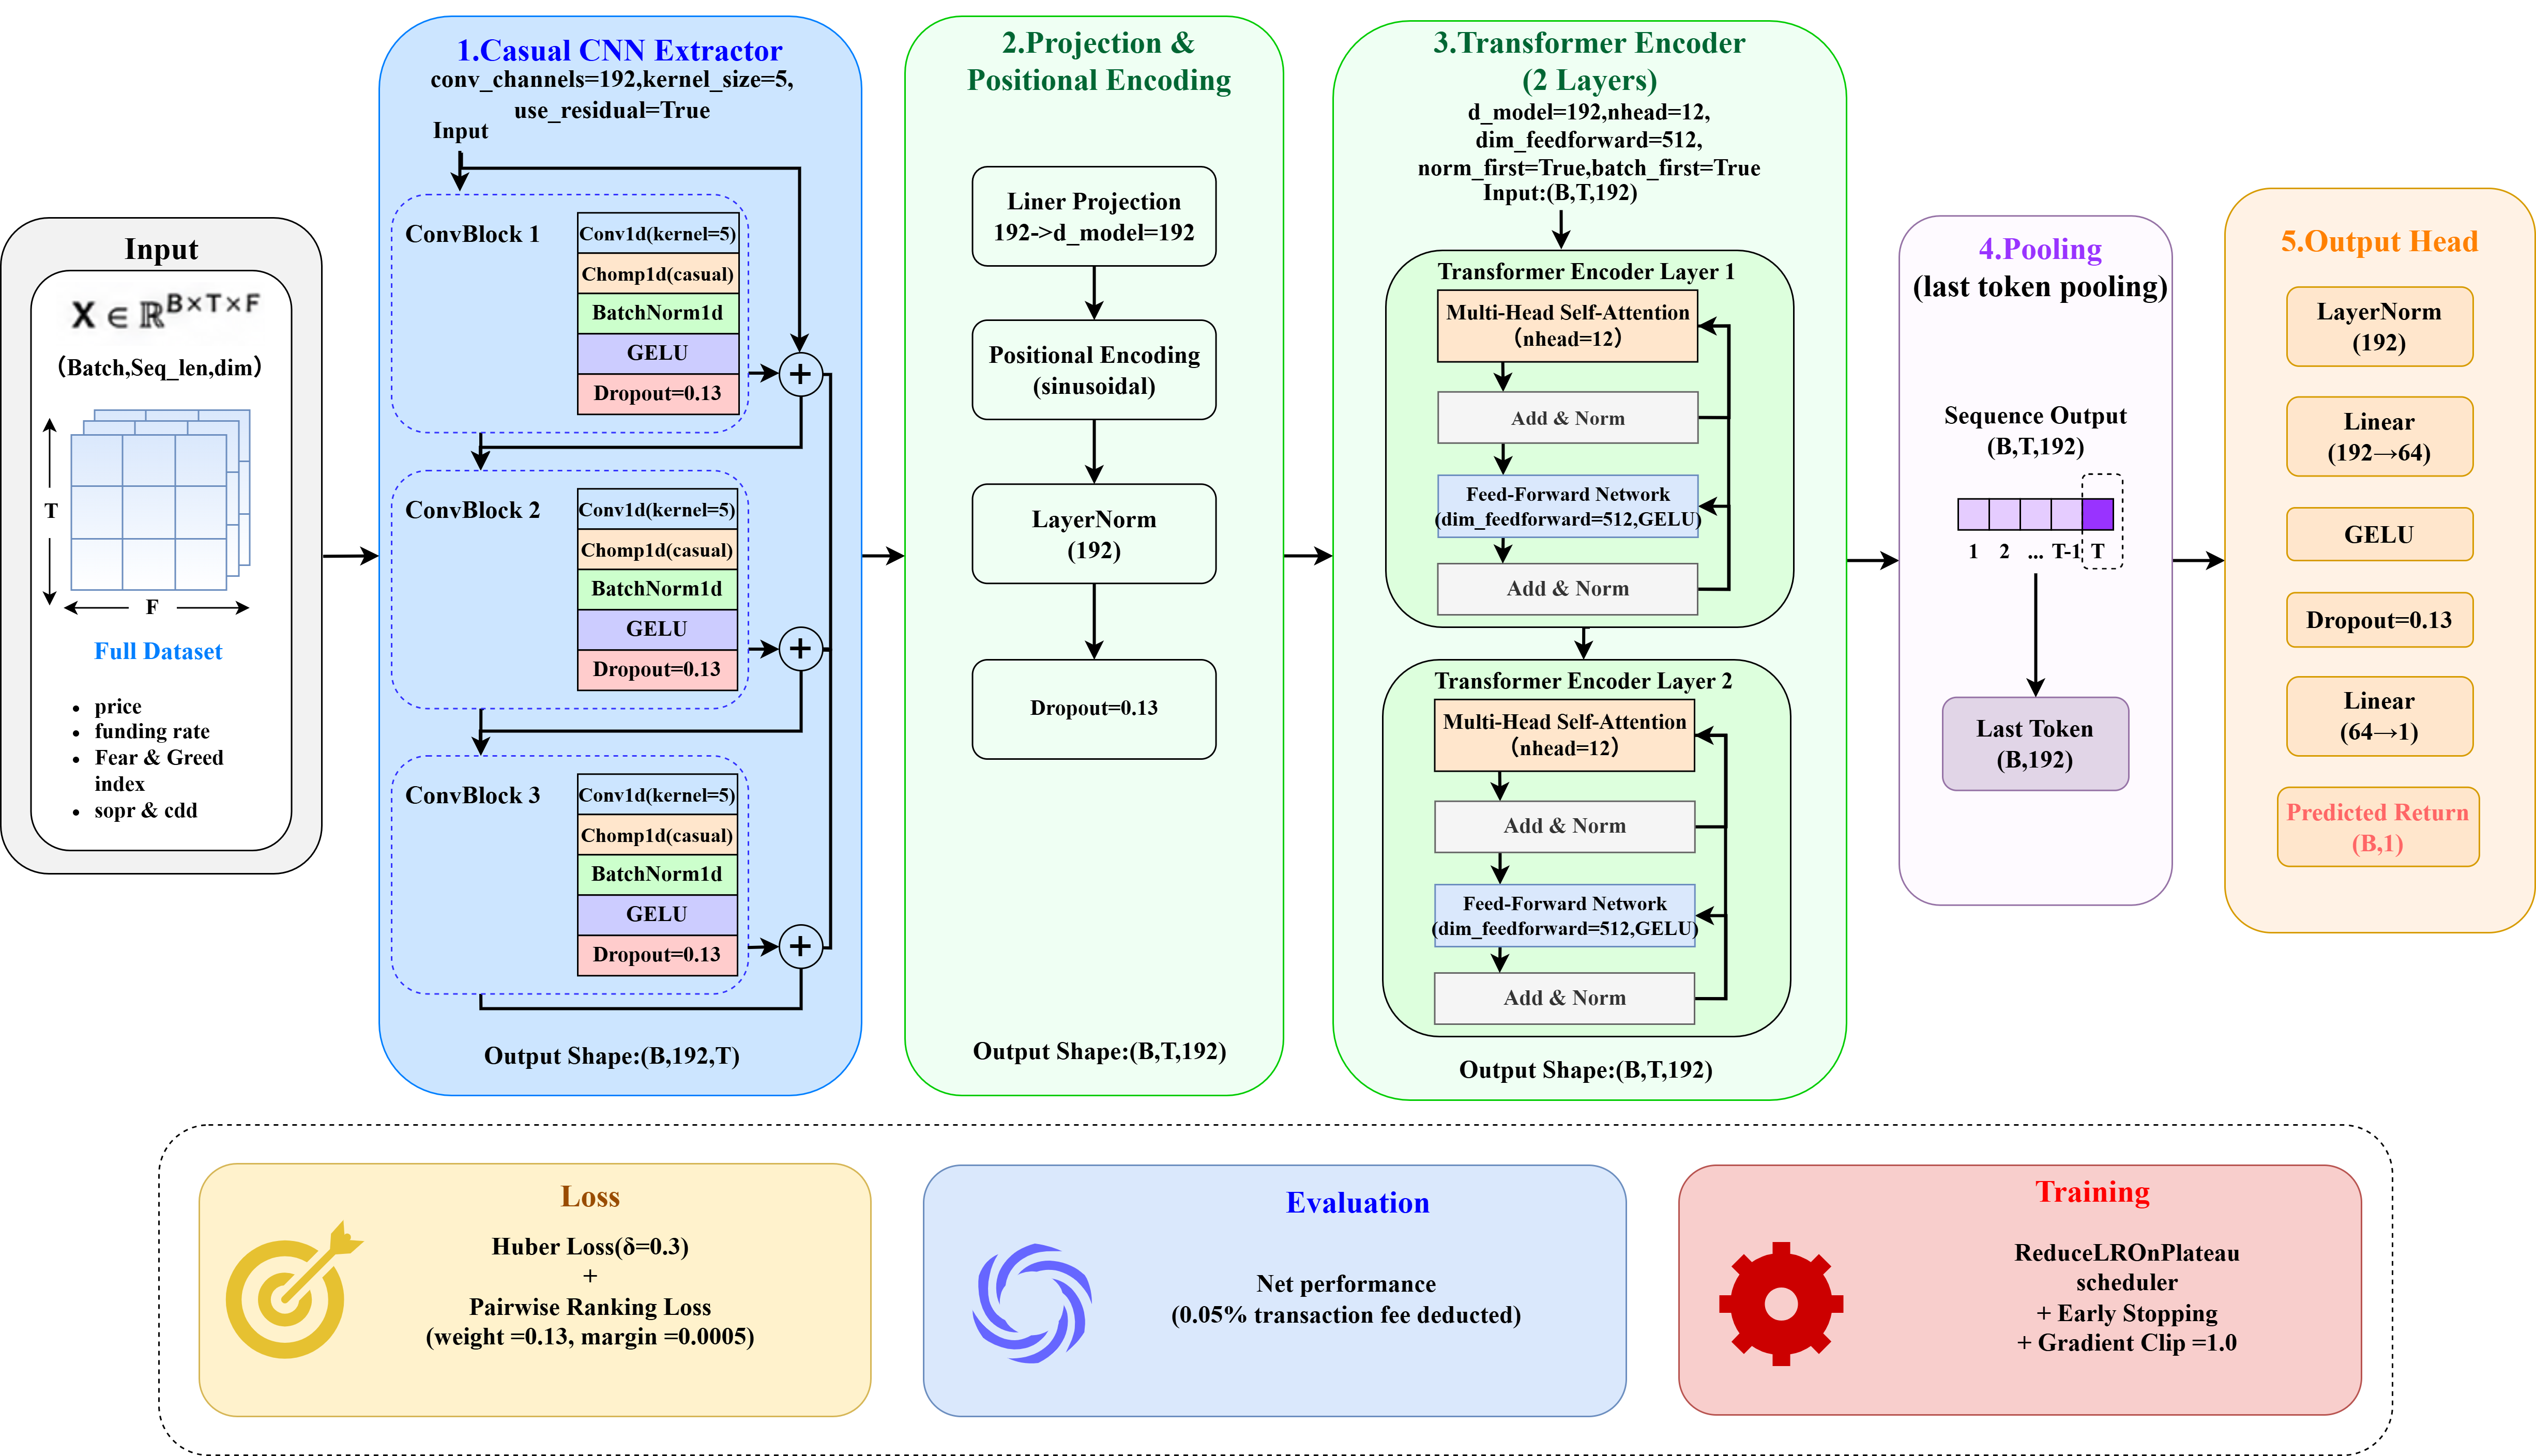
\includegraphics[width=0.78\textwidth]{../charts/CNN-Transformer.png}
\caption{CNN-Transformer architecture: the input sequence passes through three layers of causal convolution (ConvBlock) to extract local patterns, followed by a Transformer encoder to capture long-range dependencies, and finally a pooling layer outputs the log-return prediction.}
\label{fig:cnn_transformer_arch}
\end{figure*}

\subsection{Loss Function Design}

Drawing on the learning-to-rank paradigm from quantitative finance, this paper designs a composite loss function that balances absolute prediction accuracy with relative ordering among samples. The total loss is:

\begin{equation}
\mathcal{L} = (1 - \lambda_{\text{rank}}) \cdot \mathcal{L}_{\text{Huber}} + \lambda_{\text{rank}} \cdot \mathcal{L}_{\text{Ranking}}
\end{equation}

where $\mathcal{L}_{\text{Huber}}$ is the Huber loss ($\delta=0.3$), robust to extreme outliers, and $\mathcal{L}_{\text{Ranking}}$ is the Margin Ranking Loss:

\begin{equation}
\begin{split}
\mathcal{L}_{\text{Ranking}} = \frac{1}{N}\sum_{(i,j)} \max\big(0,\; &-\text{sign}(y_i - y_j) \\
&\cdot\; (\hat{y}_i - \hat{y}_j) + m\big)
\end{split}
\end{equation}

This loss penalizes sample pairs whose predicted ordering contradicts the true ordering, with $m=0.0005$ as the ranking margin. In quantitative trading, accurate relative ranking is often more important than precise absolute values; as long as the predicted direction is correct, the strategy can generate profits. The ranking loss weight $\lambda_{\text{rank}}=0.13$. All three hyperparameters ($\delta$, $\lambda_{\text{rank}}$, $m$) were determined via grid search on the validation set, selecting the combination with the lowest validation loss.

\subsection{Training Configuration}

All deep learning models share a unified training setup: batch size 64, AdamW optimizer, weight decay 1e-4, maximum 200 epochs, early stopping patience of 20 epochs, ReduceLROnPlateau learning rate scheduler (mode='min', factor=0.5, patience=10), and gradient clipping threshold 1.0. Predictions are clipped to $[-0.005, 0.005]$ during evaluation to mitigate the impact of extreme predictions on strategy metrics.

\section{Experimental Design}

\subsection{Evaluation Metrics}

This paper establishes a two-dimensional evaluation framework encompassing predictive ability and strategy performance. The predictive ability dimension includes:

\begin{itemize}[leftmargin=1.5em]
    \item Rank IC (IC): Spearman rank correlation coefficient between predictions and true values, measuring ranking accuracy.
    \item Pearson IC (PIC): Pearson linear correlation coefficient between predictions and true values.
    \item Directional Accuracy (DA): Fraction of samples where the predicted sign (positive/negative) matches the true sign.
    \item Mean Squared Error (MSE): Mean squared error between predictions and true values.
\end{itemize}

The strategy performance dimension is based on a simulated trading strategy: go long when the prediction is positive and go short when negative, with position size $\text{sign}(\hat{y})$, incorporating 0.05\% (5 bps) round-trip transaction cost. The following are computed:

\begin{itemize}[leftmargin=1.5em]
    \item Sharpe Ratio: Annualized Sharpe ratio, where 2190 is the number of 4-hour periods per year.
    \item Information Ratio (IR): Ratio of the mean to standard deviation of rolling 48-period Rank IC, measuring signal consistency \cite{grinold2000}.
    \item Maximum Drawdown (MaxDD): Magnitude of the maximum drawdown of the simulated equity curve.
    \item Annual Return: Annualized average strategy return.
\end{itemize}

\subsection{Experiment Setup}

Four groups of experiments are designed:

\medskip
\noindent Exp.~1 (Full-set model comparison). Compare all 10 models on the full feature set to examine the predictive ability of different architectures.

\smallskip
\noindent Exp.~2 (Feature ablation). Train all 10 models on each of the 6 feature configurations to analyze the marginal contribution of different data sources.

\smallskip
\noindent Exp.~3 (Multi-seed stability analysis). Replicate experiments with 5 different random seeds (0, 1, 2, 42, 123) to verify statistical reliability.

\smallskip
\noindent Exp.~4 (Sliding window validation). Employ fixed-size sliding windows (2-year training / 6-month testing / 6-month step, 8 windows total) on the full feature set, training all 10 models to test temporal robustness across market regimes. This experiment uses seed=1.

\section{Experimental Results and Analysis}

\subsection{Full-Set Model Comparison}

Table~\ref{tab:full_results} presents complete test-set evaluation results for all 10 models on the full feature set (seed=1).

\begin{table*}[t]
\centering
\footnotesize
\caption{Test-set performance comparison across models on the full feature set (seed=1)}
\label{tab:full_results}
\begin{tabular}{lcccccccc}
\toprule
Model & IC & PIC & DA & MSE & Sharpe & IR & MaxDD & AnnRet \\
\midrule
CNN-Transformer & \textbf{0.149} & \textbf{0.163} & \textbf{0.549} & 0.0001 & \textbf{5.652} & \textbf{1.125} & 0.186 & \textbf{2.306} \\
LSTM-Transformer & 0.108 & 0.131 & 0.530 & 0.0001 & 3.259 & 0.865 & 0.255 & 1.334 \\
Transformer & 0.135 & 0.151 & 0.545 & 0.0001 & 4.333 & 0.989 & 0.207 & 1.773 \\
LSTM & 0.119 & 0.120 & 0.519 & 0.0001 & 2.257 & 0.992 & 0.291 & 0.925 \\
TCN & 0.062 & 0.085 & 0.512 & 0.0001 & 0.050 & 0.494 & 0.366 & 0.021 \\
ModernTCN & 0.063 & 0.083 & 0.513 & 0.0001 & 0.168 & 0.455 & 0.415 & 0.069 \\
PatchTST & 0.128 & 0.145 & 0.532 & 0.0001 & 3.981 & 0.867 & 0.261 & 1.630 \\
XGBoost & 0.128 & 0.144 & 0.542 & 0.0001 & 4.496 & 0.885 & 0.183 & 1.838 \\
TimeMixer & 0.115 & 0.147 & 0.524 & 0.0001 & 1.781 & 0.790 & 0.321 & 0.730 \\
DLinear & 0.051 & 0.063 & 0.520 & 0.0001 & $-0.464$ & 0.331 & 0.490 & $-0.191$ \\
\midrule
Buy \& Hold & -- & -- & -- & -- & $-0.710$ & -- & 0.518 & $-0.292$ \\
Simple Momentum & -- & -- & 0.481 & -- & 0.290 & -- & -- & 0.119 \\
\bottomrule
\end{tabular}
\end{table*}

All 10 models substantially outperform naive baselines (Buy \& Hold Sharpe $-0.71$), ruling out mere market beta exposure.

(1) The CNN-Transformer achieves the best numerical performance. CNN-Transformer attains Sharpe=5.65, IC=0.149. Transformer (4.33), XGBoost (4.50), PatchTST (3.98), and LSTM-Transformer (3.26) also produce strong results. XGBoost's high static Sharpe is not reproducible under sliding windows (Section~6.6). DLinear, as the linear baseline, records a negative test Sharpe ($-0.46$), confirming that simple linear decomposition cannot extract effective signals in this multi-source, low-SNR setting. TimeMixer (ICLR 2024) achieves a test Sharpe of only 1.78 on the full set, substantially weaker than its performance on price\_funding\_fng (4.89)---this sharp decay ($\Delta$Sharpe $-3.11$) reveals that even state-of-the-art multi-scale mixing architectures cannot exploit on-chain data without the CNN-Transformer's hierarchical feature extraction pipeline. ModernTCN and TCN exhibit severe train-test gaps (e.g., ModernTCN training Sharpe reaches 19.30 vs.\ test 0.17).

(2) Small IC improvements nonlinearly amplify into substantial Sharpe gains. The modest IC difference between CNN-Transformer and Transformer (0.149 vs.\ 0.135) translates into an economically meaningful Sharpe gap (5.65 vs.\ 4.33).

\begin{figure*}[t]
\centering
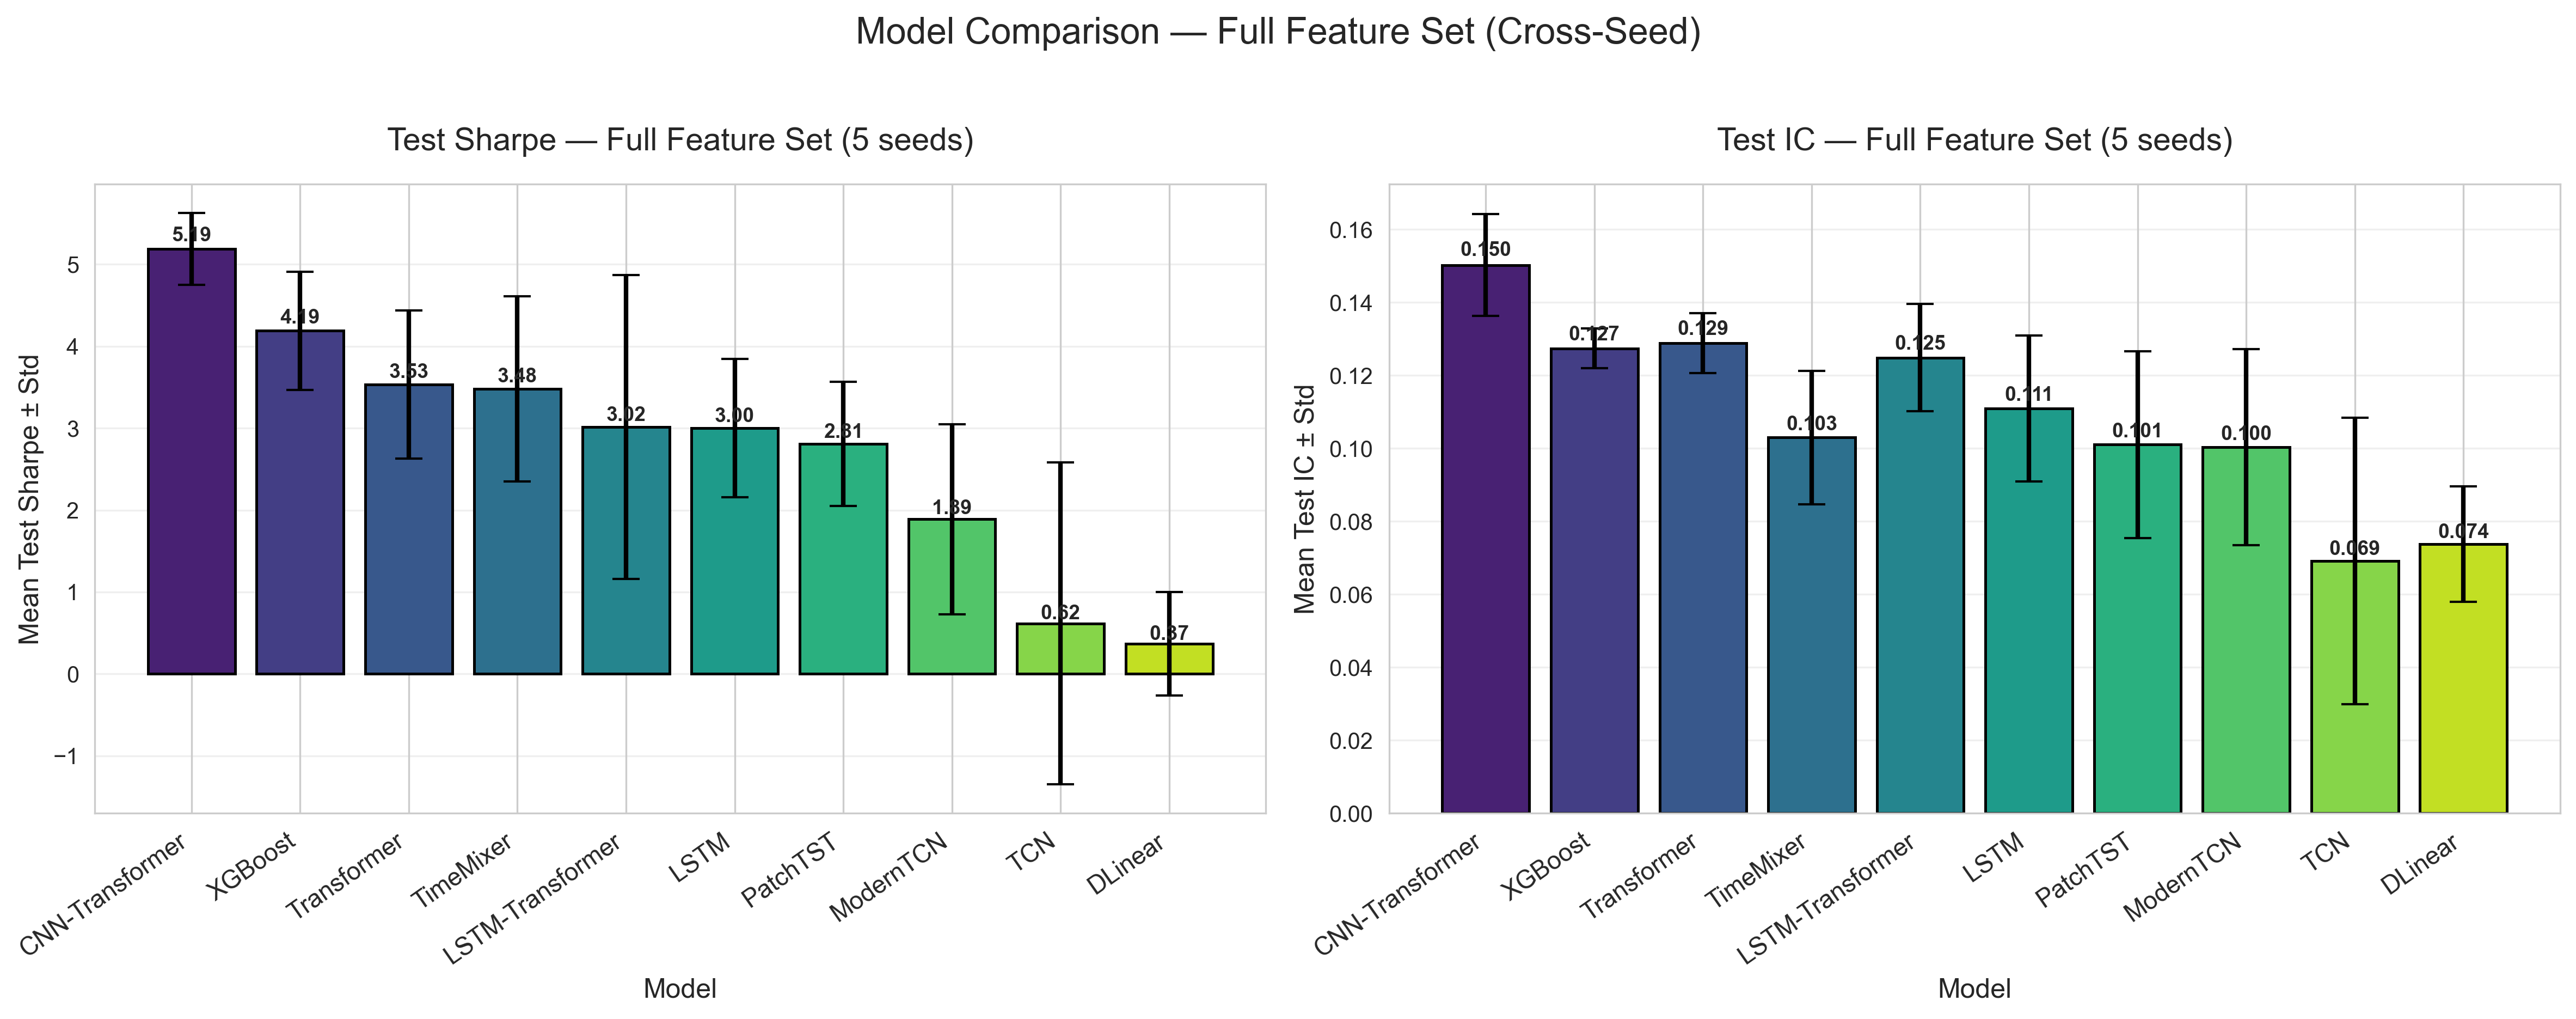
\includegraphics[width=0.80\textwidth]{../charts/model_comparison_full.png}
\caption{Cross-5-seed test Sharpe and IC comparison across models on the full feature set (mean $\pm$ std)}
\label{fig:model_comparison}
\end{figure*}

\subsection{Feature Ablation Experiment}

Table~\ref{tab:feature_ablation} shows the test-set Sharpe ratios across all 10 models under the 6 feature configurations, along with each model's cross-feature-set ranking.

\begin{table*}[t]
\centering
\footnotesize
\setlength{\tabcolsep}{2.5pt}
\caption{Test-set Sharpe ratio comparison across models under six feature configurations (seed=1)}
\label{tab:feature_ablation}
\begin{tabular}{lcccccccc}
\toprule
\multirow{2}{*}{Model} & \multicolumn{6}{c}{Feature Configuration} & \multirow{2}{*}{Mean} & \multirow{2}{*}{Std} \\
\cmidrule(lr){2-7}
& only & fund & fng & onch & lon & full \\
\midrule
CNN-Transformer & $-2.27$ & $-2.52$ & 2.20 & $-0.85$ & $-2.90$ & \textbf{5.65} & $-0.11$ & 3.26 \\
Transformer & $-1.94$ & $-2.00$ & 4.37 & $-1.42$ & $-2.70$ & \textbf{4.33} & 0.11 & 3.14 \\
LSTM & $-1.10$ & $-0.19$ & 4.28 & $-2.01$ & $-1.87$ & \textbf{2.26} & 0.23 & 2.60 \\
LSTM-Transformer & $-0.07$ & $-0.81$ & 0.46 & $-0.94$ & $-1.94$ & \textbf{3.26} & $-0.01$ & 1.81 \\
TCN & $-2.79$ & $-3.31$ & 1.75 & $-3.11$ & $-2.76$ & \textbf{0.05} & $-1.70$ & 2.36 \\
ModernTCN & $-2.35$ & $-1.20$ & 2.39 & $-3.69$ & $-0.61$ & \textbf{0.17} & $-0.88$ & 2.10 \\
PatchTST & $-1.44$ & $-3.29$ & 3.52 & $-0.73$ & $-2.68$ & \textbf{3.98} & $-0.11$ & 3.12 \\
XGBoost & -- & -- & 4.50 & -- & -- & \textbf{4.50} & -- & -- \\
TimeMixer & $-1.46$ & $-0.44$ & \textbf{4.89} & $-0.71$ & $-1.63$ & 1.78 & 0.41 & 2.72 \\
DLinear & $-2.72$ & $-2.66$ & 0.82 & $-2.68$ & $-2.83$ & $-0.46$ & $-1.75$ & 1.52 \\
\bottomrule
\multicolumn{9}{p{0.9\textwidth}}{\footnotesize Note: only=price\_only; fund=price\_funding; fng=price\_funding\_fng; onch=price\_onchain; lon=price\_long\_onchain; full=all features. XGBoost produced no predictive signal on other feature sets (IC=0), denoted by ``--''. DLinear achieves a positive Sharpe only on price\_funding\_fng (0.82) but is significantly weaker than deep models; TimeMixer reaches the highest Sharpe (4.89) on price\_funding\_fng but decays sharply when on-chain data is added ($\Delta$Sharpe $-3.11$).}
\end{tabular}
\end{table*}

Table~\ref{tab:feature_ablation} reveals a striking pattern: on-chain data is simultaneously useless in isolation and powerful in combination.

When on-chain indicators appear alone alongside only price features, they do not yield a positive test Sharpe for any model. Both price\_onchain and price\_long\_onchain fail to produce positive returns across all 10 models. The CNN-Transformer, for instance, sees its Sharpe improve from $-2.27$ to $-0.85$ (an improvement, but still negative), whereas LSTM, TCN, and ModernTCN actually degrade (e.g., TCN drops from $-2.79$ to $-3.11$). The likely explanation is threefold: on-chain fluctuation logic operates at daily or lower frequencies, mismatching the 4-hour granularity; on-chain transaction randomness masks systematic signals; and short-term price movements are driven primarily by derivatives market dynamics rather than on-chain supply-demand forces.

The picture shifts markedly once derivative and sentiment features are present. Table~\ref{tab:onchain_synergy} contrasts the Sharpe changes from price\_funding\_fng to full for each model.

\begin{table*}[t]
\centering
\caption{On-chain data synergy: Sharpe ratio change from price\_funding\_fng to full (seed=1)}
\label{tab:onchain_synergy}
\small
\begin{tabular}{lcccc}
\toprule
Model & Sharpe$_{\text{fng}}$ & Sharpe$_{\text{full}}$ & $\Delta$Sharpe & Synergy Type \\
\midrule
CNN-Transformer & 2.20 & 5.65 & +3.45 & Strong positive \\
LSTM-Transformer & 0.46 & 3.26 & +2.80 & Strong positive \\
PatchTST & 3.52 & 3.98 & +0.46 & Weak positive \\
Transformer & 4.37 & 4.33 & $-0.04$ & Neutral \\
XGBoost & 4.50 & 4.50 & 0.00 & Completely ignores \\
LSTM & 4.28 & 2.26 & $-2.02$ & Negative interference \\
TCN & 1.75 & 0.05 & $-1.70$ & Negative interference \\
ModernTCN & 2.39 & 0.17 & $-2.22$ & Negative interference \\
TimeMixer & \textbf{4.89} & 1.78 & \textbf{$-3.11$} & Strong negative \\
DLinear & 0.82 & $-0.46$ & $-1.28$ & Weak negative / near neutral \\
\bottomrule
\end{tabular}
\end{table*}

The CNN-Transformer gains 3.45 Sharpe points (2.20$\to$5.65), and the LSTM-Transformer gains 2.80 (0.46$\to$3.26). Yet the same on-chain features hurt LSTM, TCN, and ModernTCN, leave Transformer and PatchTST essentially unchanged, and are entirely ignored by XGBoost. Most strikingly, TimeMixer collapses: it leads all models with Sharpe=4.89 on price\_funding\_fng, yet plummets to 1.78 ($\Delta$Sharpe $-3.11$) because its cross-scale mixing operates on the time rather than the feature dimension, lacking explicit cross-source modeling.

These outcomes map cleanly onto architectural families, forming three groups:

\begin{itemize}[leftmargin=1.5em]
    \item Synergistic utilization ($\Delta$Sharpe $> +2$): CNN-Transformer, LSTM-Transformer. Hybrid architectures with hierarchical representation---local pattern extraction followed by cross-feature attention---naturally suit cross-source interaction.
    \item Neutral ($\Delta$Sharpe $\approx 0$): Transformer, PatchTST, DLinear, XGBoost. Pure self-attention treats all dimensions equally; DLinear's linear decomposition barely responds to on-chain features ($\Delta$Sharpe $-1.28$); XGBoost's greedy feature selection ignores them entirely.
    \item Negative interference ($\Delta$Sharpe $< -1.5$): LSTM, TCN, ModernTCN, TimeMixer. Pure recurrent/convolutional architectures lack explicit cross-feature attention, so on-chain noise overwhelms the occasional strong signals.
\end{itemize}

The gain fundamentally arises from learned interaction flexibility: rather than locking cross-source interactions into fixed hand-crafted products, raw on-chain features allow the attention mechanism to data-dependently discover conditional feature pairings. The CNN-Transformer's hierarchical pipeline---causal convolutions for local temporal patterns, multi-head self-attention for global cross-source dependencies---uniquely enables this capability. On-chain data demonstrates meaningful predictive power only when three conditions align: the right indicator type (short-term SOPR/CDD), the right companion data sources (funding rate and sentiment), and the right architecture (CNN/LSTM + Transformer hybrid).

price\_only cannot produce profitable trading strategies. When using only price data, none of the 10 models achieve a positive test Sharpe---the signal strength is insufficient to produce a positive Sharpe ratio after deducting transaction costs.

\begin{figure*}[t]
\centering
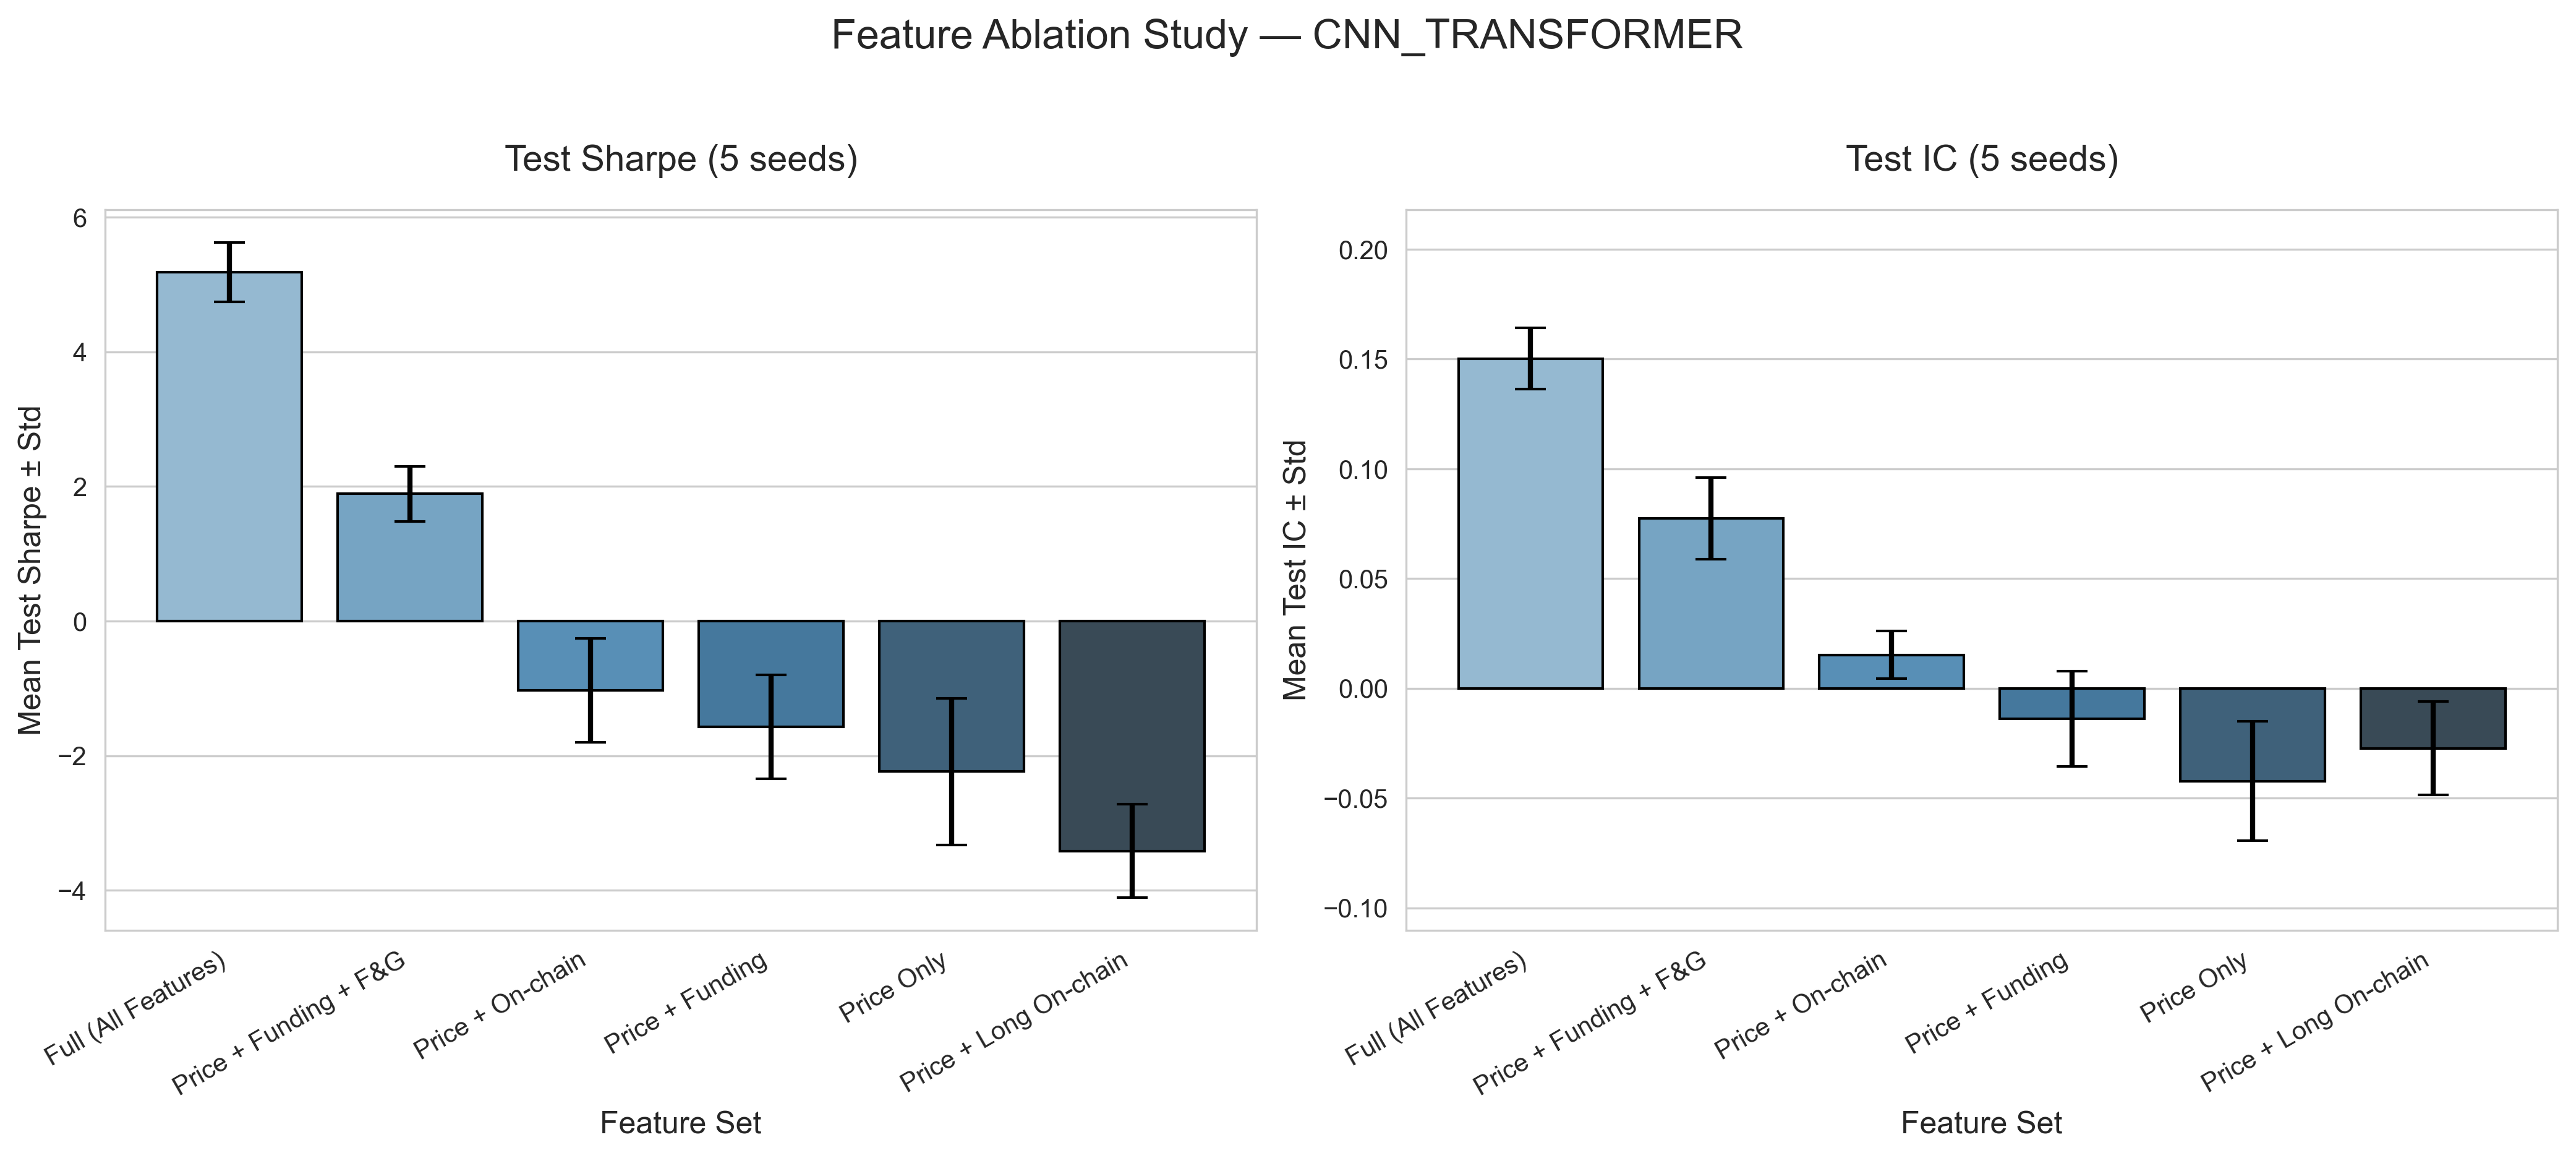
\includegraphics[width=0.80\textwidth]{../charts/feature_ablation_cnn_transformer.png}
\caption{CNN-Transformer test Sharpe and IC across six feature configurations (5-seed mean $\pm$ std)}
\label{fig:feature_ablation}
\end{figure*}

\subsubsection{Prediction Accuracy Dimension: MSE Feature Ablation Analysis}

The preceding ablation analysis is based on strategy-level metrics such as the Sharpe ratio. This subsection provides a complementary perspective from the standpoint of \textbf{pure prediction accuracy} (MSE). Table~\ref{tab:mse_ablation} presents the test-set MSE for all 10 models under the six feature configurations (seed=1, multiplied by $10^{4}$ for readability), along with the MSE change from price\_funding\_fng to full ($\Delta$MSE, where a negative value indicates reduced prediction error after adding on-chain data).

% MSE-based feature ablation (English)
\begin{table*}[t]
\centering
\footnotesize
\setlength{\tabcolsep}{1.5pt}
\caption{Test-set MSE comparison across models under six feature configurations (seed=1, $\times 10^{4}$)}
\label{tab:mse_ablation}
\begin{tabular}{lccccccc}
\toprule
\multirow{2}{*}{Model} & \multicolumn{6}{c}{Feature Configuration (MSE $\times 10^{4}$)} & \multirow{2}{*}{$\Delta$MSE} \\
\cmidrule(lr){2-7}
& only & fund & fng & onch & lon & full \\
\midrule
CNN-Transformer & 0.77 & 0.77 & 0.77 & 0.77 & 0.77 & \textbf{0.75} & \textbf{$-0.02$} \\
PatchTST & 0.77 & 0.78 & 0.78 & 0.77 & 0.77 & 0.75 & $-0.03$ \\
LSTM-Transformer & 0.77 & 0.77 & 0.77 & 0.77 & 0.77 & 0.76 & $-0.01$ \\
XGBoost & 0.77 & 0.77 & 0.76 & 0.77 & 0.77 & 0.76 & 0.00 \\
TCN & 0.77 & 0.78 & 0.76 & 0.77 & 0.78 & 0.77 & $+0.01$ \\
ModernTCN & 0.77 & 0.77 & 0.77 & 0.78 & 0.77 & 0.77 & 0.00 \\
TimeMixer & 0.77 & 0.77 & \textbf{0.75} & 0.77 & 0.77 & 0.77 & $+0.02$ \\
LSTM & 0.77 & 0.77 & 0.76 & 0.77 & 0.77 & 0.77 & $+0.01$ \\
Transformer & 0.78 & 0.79 & 0.78 & 0.80 & 0.79 & 0.77 & $-0.01$ \\
DLinear & 0.79 & 0.78 & 0.78 & 0.80 & 0.79 & 0.80 & $+0.02$ \\
\bottomrule
\multicolumn{8}{p{0.85\textwidth}}{\footnotesize only=price\_only; fund=price\_funding; fng=price\_funding\_fng; onch=price\_onchain; lon=price\_long\_onchain. $\Delta$MSE = MSE$_{\text{full}}$ $-$ MSE$_{\text{fng}}$ (negative = on-chain data reduces prediction error). Bold indicates the best value in each column. TimeMixer achieves the lowest MSE (0.75) on the fng set, but its MSE increases to 0.77 after adding on-chain data ($\Delta$+0.02, tied worst with DLinear).}
\end{tabular}
\end{table*}


From Table~\ref{tab:mse_ablation}, the following observations emerge: \textbf{(1) MSE differences are extremely small in magnitude.} The test MSE across all models and feature sets is concentrated within the narrow range of $0.75$--$0.80\times10^{-4}$ (a maximum difference of only $0.05\times10^{-4}$), explaining why evaluation approaches that rely solely on MSE in the literature struggle to distinguish models. \textbf{(2) MSE changes and Sharpe changes move in the same direction.} CNN-Transformer achieves the lowest MSE on the full set (0.75), with on-chain data simultaneously improving both prediction accuracy and strategy returns; TimeMixer's MSE rebounds after adding on-chain data ($\Delta$+0.02), fully consistent with its $\Delta$Sharpe of $-3.11$. \textbf{(3) MSE and Sharpe exhibit a nonlinear mapping.} CNN-Transformer and TimeMixer differ by only 0.02 in MSE on the fng set, yet their Sharpe gap on the full set reaches 3.87---a small accuracy difference is nonlinearly amplified into a large strategy return gap, providing quantitative evidence that pure accuracy metrics are insufficient substitutes for strategy metrics in financial forecasting.

\subsection{Multi-Seed Stability Analysis}

To exclude the influence of single-seed randomness on conclusions, this paper replicates all experiments on the full feature set across 5 different random seeds (0, 1, 2, 42, 123). Table~\ref{tab:multi_seed} presents cross-seed statistics.

\begin{table*}[t]
\centering
\caption{Cross-5-seed test-set performance statistics on the full feature set (mean $\pm$ std)}
\label{tab:multi_seed}
\small
\begin{tabular}{lcccc}
\toprule
Model & IC & Sharpe & MaxDD & AnnRet \\
\midrule
CNN-Transformer & 0.150$\pm$0.014 & 5.187$\pm$0.441 & 0.174$\pm$0.038 & 2.115$\pm$0.177 \\
Transformer & 0.129$\pm$0.008 & 3.531$\pm$0.903 & 0.198$\pm$0.021 & 1.446$\pm$0.367 \\
LSTM-Transformer & 0.125$\pm$0.015 & 3.016$\pm$1.855 & 0.253$\pm$0.144 & 1.234$\pm$0.759 \\
LSTM & 0.111$\pm$0.020 & 3.000$\pm$0.844 & 0.234$\pm$0.035 & 1.228$\pm$0.344 \\
PatchTST & 0.101$\pm$0.026 & 2.807$\pm$0.758 & 0.258$\pm$0.042 & 1.150$\pm$0.309 \\
XGBoost & 0.127$\pm$0.005 & 4.189$\pm$0.720 & 0.204$\pm$0.029 & 1.713$\pm$0.293 \\
TCN & 0.069$\pm$0.039 & 0.616$\pm$1.966 & 0.386$\pm$0.218 & 0.252$\pm$0.807 \\
ModernTCN & 0.100$\pm$0.027 & 1.888$\pm$1.162 & 0.286$\pm$0.084 & 0.775$\pm$0.477 \\
TimeMixer & 0.103$\pm$0.018 & 3.480$\pm$1.131 & 0.218$\pm$0.067 & 1.424$\pm$0.463 \\
DLinear & 0.074$\pm$0.016 & 0.368$\pm$0.632 & 0.378$\pm$0.071 & 0.151$\pm$0.259 \\
\bottomrule
\end{tabular}
\end{table*}

Table~\ref{tab:multi_seed} shows: (1) CNN-Transformer has the best robustness (Sharpe std 0.441, IC std 0.014). (2) Some models exhibit high seed sensitivity: LSTM-Transformer displays bimodal distribution (1/5 seeds collapses to $-0.25$, remaining 4 mean Sharpe=3.83); TimeMixer fluctuates substantially (Sharpe std 1.131); TCN (std 1.966) and ModernTCN (std 1.162) fluctuate severely. DLinear has the lowest cross-seed mean (Sharpe=0.37) among all models but with relatively controlled variance (std 0.632). (3) The on-chain synergy effect is robust---CNN-Transformer's $\Delta$Sharpe is positive across all 5 seeds (mean +3.30$\pm$0.69), while TimeMixer's $\Delta$Sharpe is positive in only 1/5 seeds (mean $-1.01$).

\subsection{Backtest Analysis}

Figure~\ref{fig:backtest1} displays backtest cumulative return curves for all ten models on the full feature set (seed=1). The CNN-Transformer achieves the best risk-adjusted performance (Sharpe=5.65, max drawdown 18.6\%), followed closely by XGBoost (Sharpe=4.50, max drawdown 18.3\%). Transformer and PatchTST perform robustly (Sharpe 4.33/3.98); LSTM-Transformer and LSTM generate positive but more volatile returns (max drawdown 25.5\%/29.1\%). TimeMixer achieves moderate positive returns (Sharpe=1.78, max drawdown 32.1\%). ModernTCN (Sharpe=0.17, max drawdown 41.5\%) and TCN (Sharpe=0.05, max drawdown 36.6\%) barely break even, with ModernTCN turning to sustained losses after brief profitable periods---in stark contrast to its extreme training-set performance. DLinear loses money throughout (Sharpe=-0.46, max drawdown 49.0\%), confirming the inadequacy of purely linear decomposition in this multi-source, low-SNR setting. The backtest ranking is fully consistent with the quantitative results in Table~\ref{tab:full_results}, further validating the three-group architecture taxonomy.

\begin{figure*}[t]
\centering
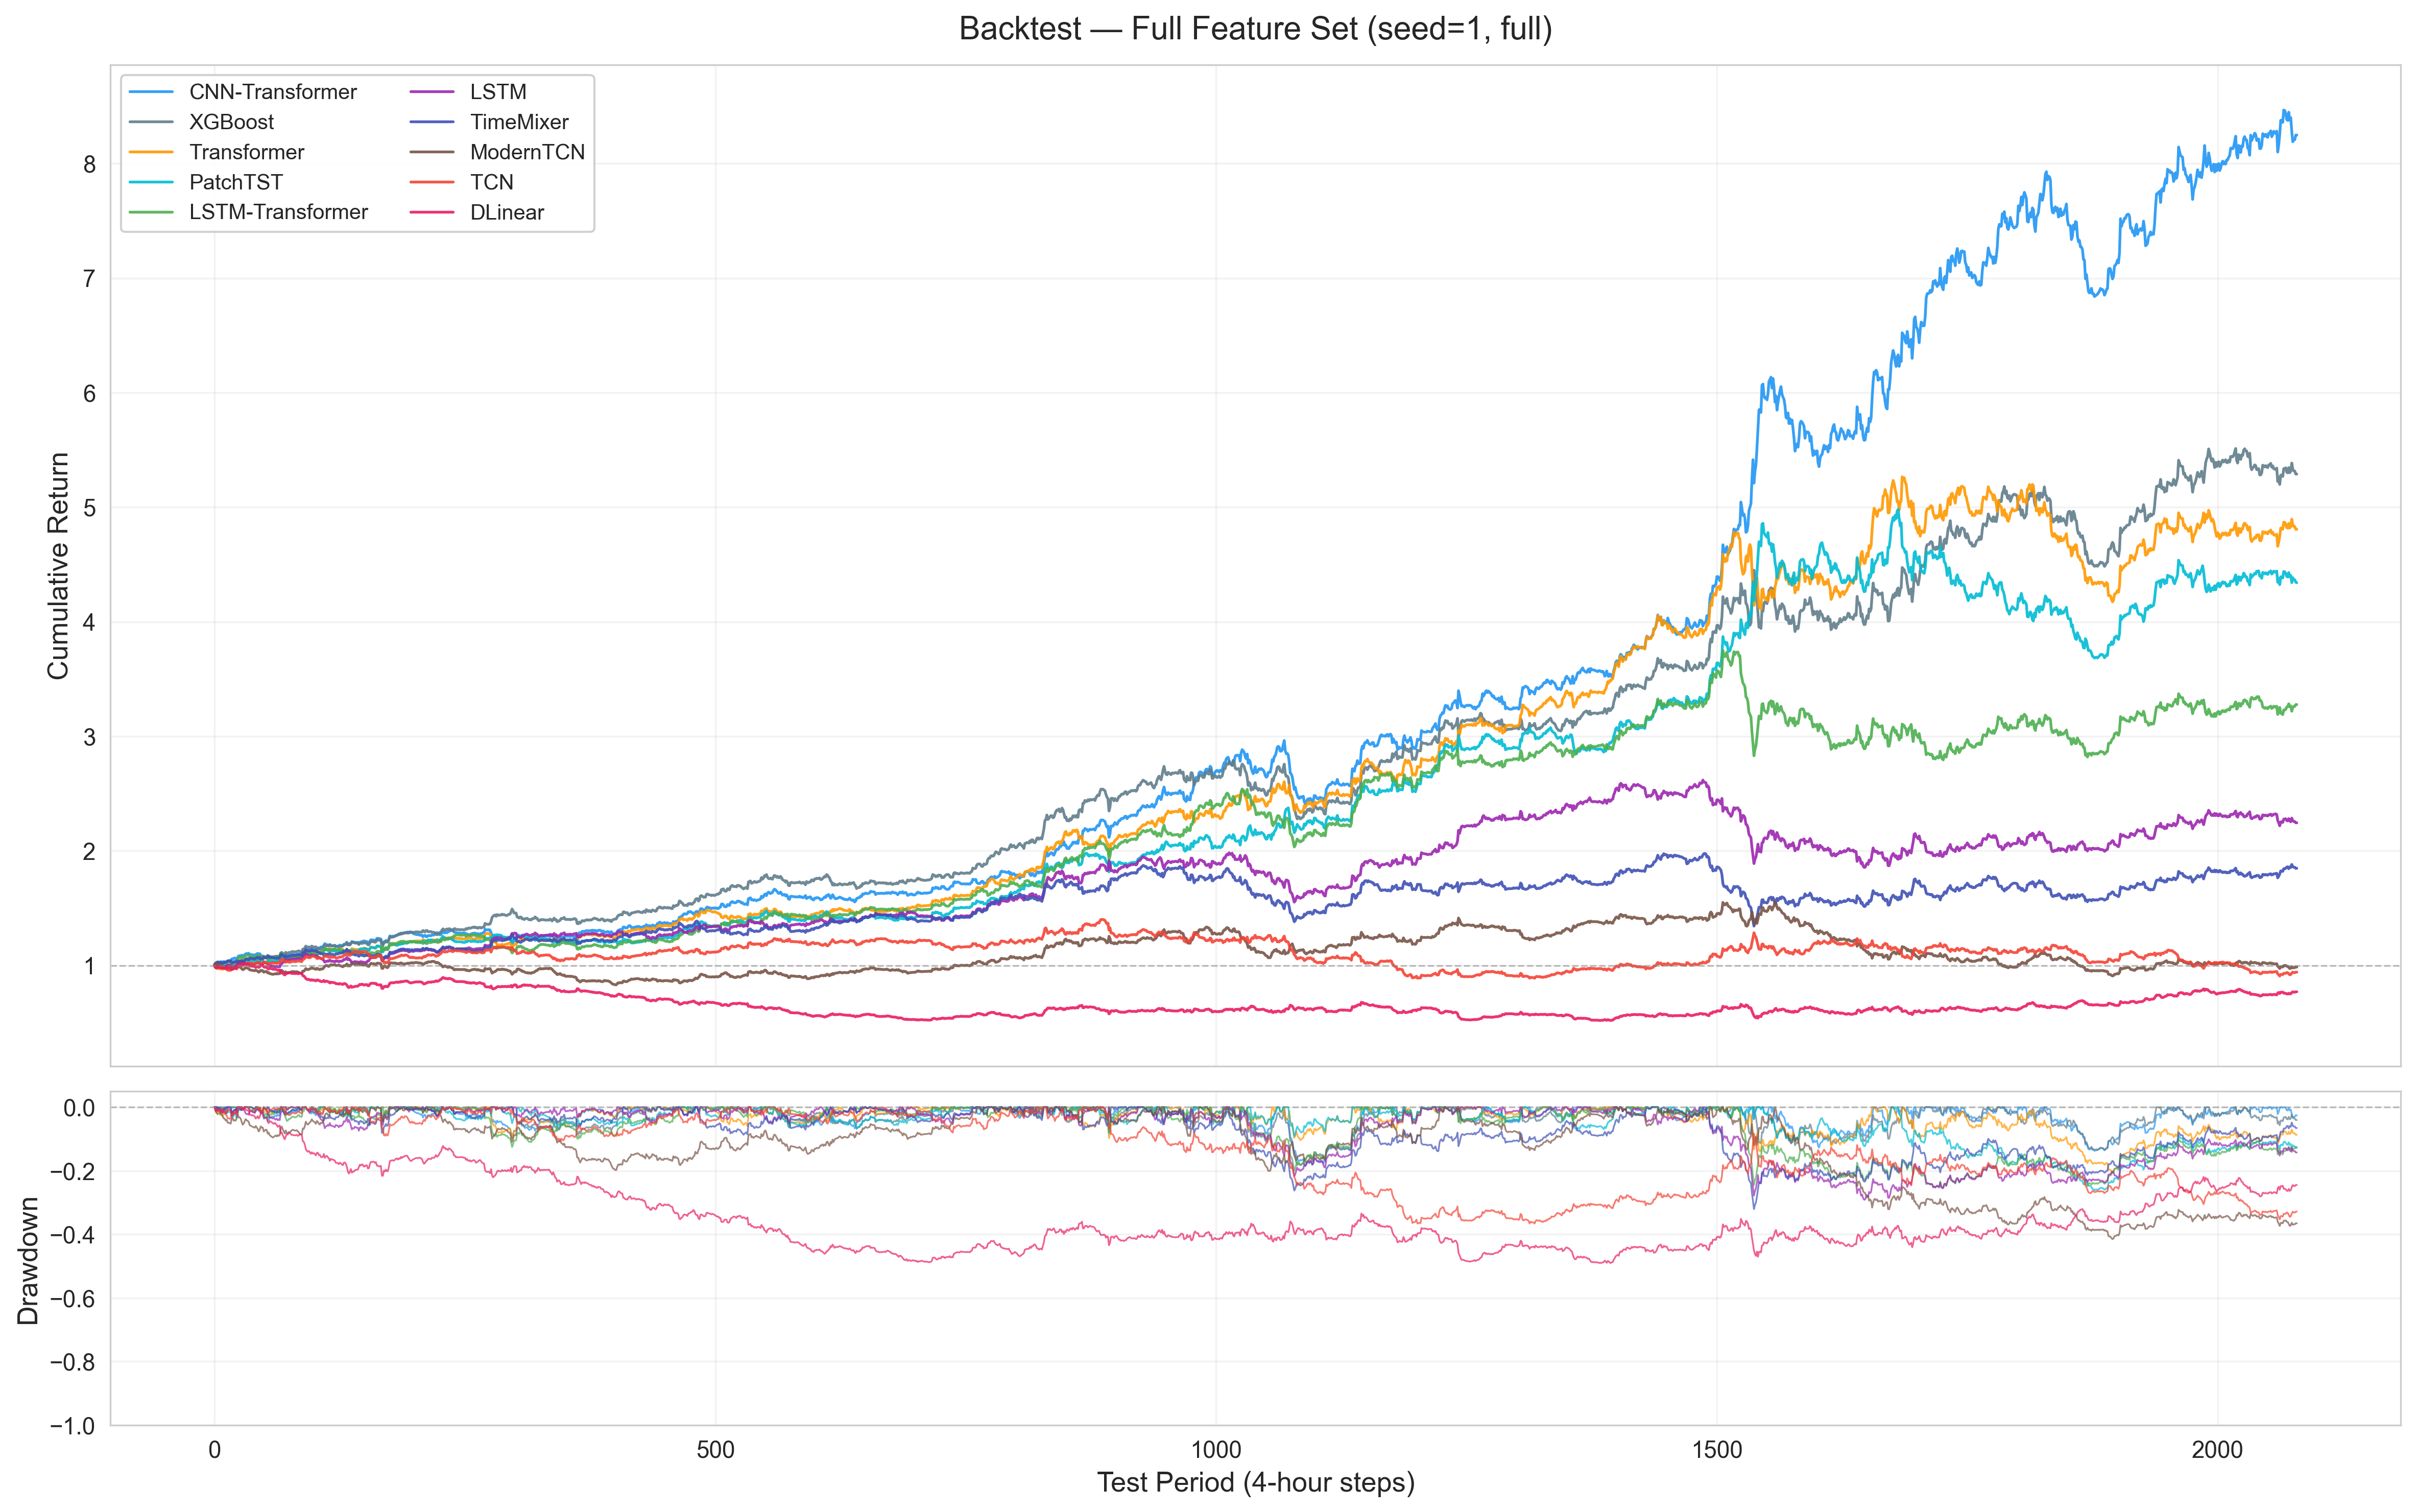
\includegraphics[width=0.88\textwidth]{../charts/backtest_full_all_models.png}
\caption{Backtest cumulative return curves for all ten models on the full feature set (seed=1)}
\label{fig:backtest1}
\end{figure*}

\subsubsection{Backtest Visualization of On-Chain Synergy}

Figure~\ref{fig:backtest_synergy} contrasts the CNN-Transformer's backtest curves across two feature sets (full vs.\ price\_funding\_fng):

\begin{figure*}[t]
\centering
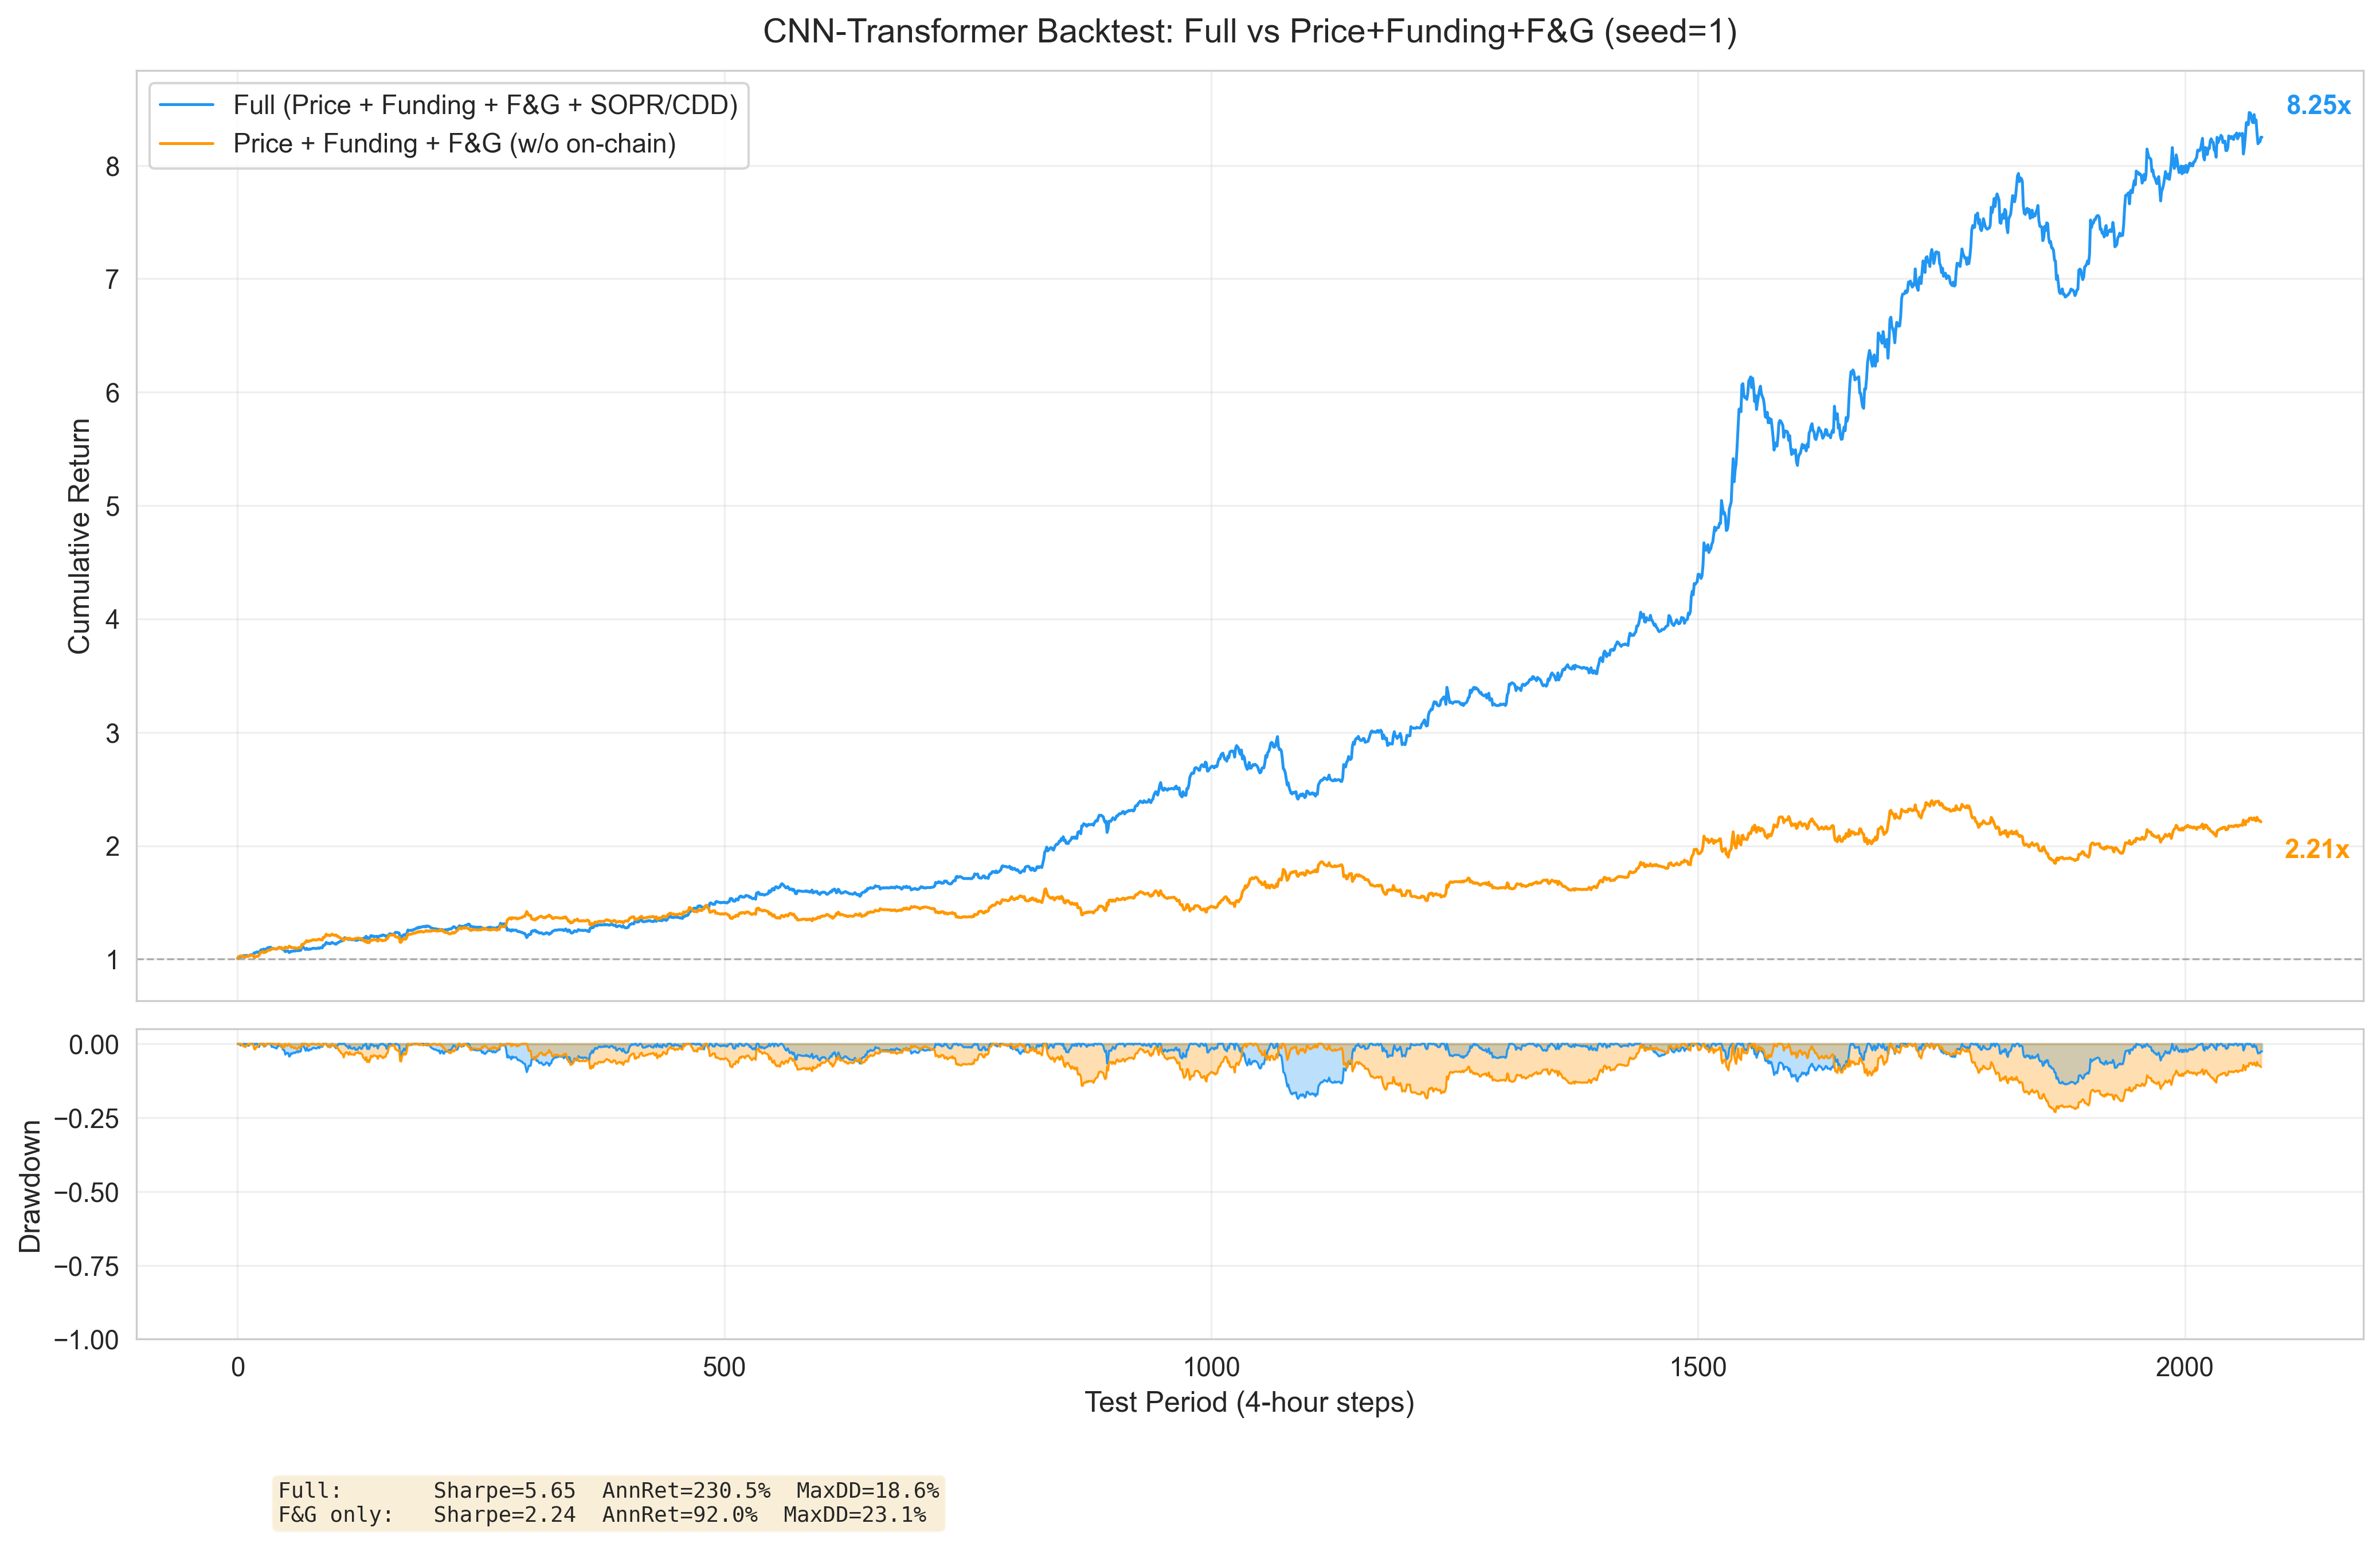
\includegraphics[width=0.88\textwidth]{../charts/backtest_synergy_full_vs_fng.png}
\caption{Backtest comparison of CNN-Transformer on full vs.\ price\_funding\_fng (seed=1). Upper panel: cumulative returns; lower panel: drawdowns. The full set (blue) improves over the fng set (orange) on all three dimensions: Sharpe (5.65 vs.\ 2.20), annual return (230.5\% vs.\ 90.2\%), and maximum drawdown (18.6\% vs.\ 23.1\%).}
\label{fig:backtest_synergy}
\end{figure*}

\begin{itemize}[leftmargin=1.5em]
    \item The full set cumulative return (8.25$\times$) is approximately 3.7 times that of fng (2.21$\times$), consistent with the attention mechanism gradually learning cross-source combinations.
    \item The full set maximum drawdown (18.6\%) is notably lower than fng (23.1\%), suggesting SOPR and CDD may provide early warning of reversals.
\end{itemize}

\subsection{Statistical Significance Tests}

The core thesis of this paper is that ``on-chain data's predictive value is conditional and architecture-dependent.'' This requires answering two progressive questions from a statistical inference perspective: (1) Does adding on-chain data significantly reduce the same model's prediction error? (2) Are performance differences between architectures statistically reliable? Accordingly, this section implements, in order: feature-set DM tests (directly testing the incremental contribution of on-chain data), an economic-loss DM test (strategy-level confirmation), and model-pair DM and Bootstrap tests (verifying the significance of architecture differences). Results below are based on cross-5-seed averaged predictions on the full feature set.

\subsubsection{DM Test of Feature-Set Ablation}

To directly test the core thesis, we conduct paired feature-set DM tests (full vs.\ price\_funding\_fng, MSE loss) for each of the 10 models. A negative DM statistic indicates that the full set (with SOPR/CDD on-chain data) achieves lower MSE, i.e., on-chain data reduces prediction error. Additionally, we test price\_funding\_fng vs.\ price\_funding (sentiment contribution) and price\_funding vs.\ price\_only (funding-rate contribution) to establish a complete feature-ablation statistical evidence chain. Results are shown in Table~\ref{tab:dm_feature_sets} and Table~\ref{tab:dm_feature_sets_full}.

% Feature-set DM tests — core thesis evidence (English)
\begin{table*}[t]
\centering
\caption{Feature-set DM test: incremental contribution of on-chain data (SOPR/CDD) to prediction accuracy}
\label{tab:dm_feature_sets}
\footnotesize
\setlength{\tabcolsep}{3pt}
\begin{tabular}{lcccccc}
\toprule
Model & Comparison & DM Mean & DM Range & $p$-mean & Sig.\ Seeds & Conclusion \\
\midrule
\bfseries CNN-Transformer & full vs price\_funding\_fng & \bfseries $-2.46$ & [$-2.89$, $-2.05$] & \bfseries 0.018 & 5/5 & \bfseries Significant (*) \\
Transformer & full vs price\_funding\_fng & $-0.61$ & [$-1.65$, $+0.58$] & 0.458 & 0/5 & Not sig. \\
LSTM-Transformer & full vs price\_funding\_fng & $-1.66$ & [$-3.30$, $+0.33$] & 0.329 & 3/5 & Not sig. \\
LSTM & full vs price\_funding\_fng & $+0.92$ & [$-1.42$, $+3.39$] & 0.261 & 1/5 & Not sig. \\
PatchTST & full vs price\_funding\_fng & $-0.67$ & [$-2.47$, $+0.46$] & 0.500 & 1/5 & Not sig. \\
XGBoost & full vs price\_funding\_fng & $+1.41$ & [$-0.39$, $+3.57$] & 0.374 & 2/5 & Not sig. \\
TCN & full vs price\_funding\_fng & $+1.67$ & [$-0.29$, $+4.49$] & 0.443 & 2/5 & Not sig. \\
ModernTCN & full vs price\_funding\_fng & $+0.09$ & [$-0.87$, $+1.62$] & 0.536 & 0/5 & Not sig. \\
DLinear & full vs price\_funding\_fng & $+1.46$ & [$+0.41$, $+2.49$] & 0.286 & 2/5 & Not sig. \\
TimeMixer & full vs price\_funding\_fng & $+2.26$ & [$+0.76$, $+4.84$] & 0.200 & 2/5 & Not sig. \\
\bottomrule
\multicolumn{7}{p{0.85\textwidth}}{\footnotesize Note: ** $p<0.01$, * $p<0.05$; a negative DM statistic indicates the full set achieves lower MSE than price\_funding\_fng (i.e., on-chain data reduces prediction error). Paired DM tests across 5 seeds (0, 1, 2, 42, 123). ``Sig.\ Seeds'' column reports the number of seeds reaching $p<0.05$ out of total valid seeds. XGBoost has usable models only on price\_funding\_fng and full feature sets; it failed to converge on the remaining configurations.} \\
\end{tabular}
\end{table*}

% Full feature-set DM test matrix (all 3 comparisons)
\begin{table*}[t]
\centering
\caption{Feature-set ablation DM tests: complete results for three progressive comparisons}
\label{tab:dm_feature_sets_full}
\footnotesize
\setlength{\tabcolsep}{2.5pt}
\begin{tabular}{lccc}
\toprule
Model & On-chain Synergy & Sentiment Contrib. & Funding-Rate Contrib. \\
\midrule
CNN-Transformer & $-2.46^{*}$ & $-1.46$ & $-0.18$ \\
Transformer & $-0.61$ & $-1.79$ & $-0.41$ \\
LSTM-Transformer & $-1.66$ & $-2.33$ & $+0.42$ \\
LSTM & $+0.92$ & $-3.32$ & $+0.64$ \\
PatchTST & $-0.67$ & $-0.70$ & $+0.04$ \\
XGBoost & $+1.41$ & $-5.12^{**}$ & $+0.00$ \\
TCN & $+1.67$ & $-2.12$ & $-0.13$ \\
ModernTCN & $+0.09$ & $-1.15$ & $-0.83$ \\
DLinear & $+1.46$ & $-0.67$ & $-0.28$ \\
TimeMixer & $+2.26$ & $-4.03^{**}$ & $-0.06$ \\
\bottomrule
\multicolumn{4}{p{0.85\textwidth}}{\footnotesize ** $p<0.01$, * $p<0.05$; each cell reports the DM statistic (cross-5-seed mean). A negative value indicates that the larger feature set achieves lower MSE. On-chain synergy = full vs.\ price\_funding\_fng; Sentiment contrib.\ = price\_funding\_fng vs.\ price\_funding; Funding-rate contrib.\ = price\_funding vs.\ price\_only.} \\
\end{tabular}
\end{table*}


From Table~\ref{tab:dm_feature_sets}, the following core findings emerge:

\textbf{(1) On-chain data's effectiveness is architecture-conditional, and only CNN-Transformer passes rigorous cross-seed significance testing.} Among all 10 models, only CNN-Transformer achieves statistically significant MSE reduction across all 5 seeds (cross-seed DM=$-2.46$, $p=0.018$; per-seed DM range [$-2.89$, $-2.05$], all $p<0.05$). LSTM-Transformer shows positive effects in 3/5 seeds but fails cross-seed consistency (DM=$-1.66$, $p=0.329$). The remaining 8 models---including ICLR 2024 SOTA TimeMixer (DM=$+2.26$)---show no significant MSE improvement, or even deterioration, when on-chain features are added. This result directly answers the paper's core question from the prediction-accuracy dimension: on-chain data is not universally predictive; its value strictly depends on whether the model architecture supports hierarchical cross-source feature processing.

\textbf{(2) Sentiment features (Fear \& Greed Index) provide the most universal and significant contribution.} The price\_funding\_fng vs.\ price\_funding DM test shows: XGBoost (DM=$-5.12$, $p<0.001$, 5/5 seeds significant), TimeMixer (DM=$-4.03$, $p=0.002$, 5/5 seeds significant), LSTM (DM=$-3.32$, $p=0.054$, 4/5 significant), and LSTM-Transformer (DM=$-2.33$, 3/5 significant) all obtain statistically significant MSE improvements from sentiment features. The value of sentiment signals in short-term cryptocurrency prediction is cross-architecture universal.

\textbf{(3) The independent contribution of funding rates is weak and inconsistent.} In the price\_funding vs.\ price\_only DM test, Transformer is the only model achieving significant improvement in a majority of seeds (3/5, DM=$-0.41$, $p=0.070$). The independent predictive information of funding-rate signals at the 4-hour frequency is limited; their value is mainly realized through joint interaction with sentiment and on-chain signals.

\textbf{(4) Feature-set DM tests and strategy Sharpe synergy form cross-validation.} Table~\ref{tab:dm_feature_sets_full}'s three progressive comparisons reveal a clear hierarchical structure: sentiment features benefit most models (universal layer), on-chain features benefit only hybrid architectures (conditional layer), and funding-rate contributions are limited and architecture-dependent (weak-signal layer). This is highly consistent with the $\Delta$Sharpe three-group taxonomy in Section~6.2---CNN-Transformer maintains consistent on-chain synergy gains across both MSE and Sharpe dimensions, providing dual statistical support from prediction accuracy and strategy performance perspectives.

\subsubsection{DM Test with Economic Loss Function}

The feature-set DM test above confirms the conditional effectiveness of on-chain data from the prediction-accuracy dimension. This subsection provides complementary evidence from the strategy-return dimension. Given that extremely small MSE magnitudes ($10^{-4}$) severely compress model differences, we implement a DM test using negative strategy returns as the economic loss function, where a negative DM statistic indicates superior strategy returns for the row model.

Table~\ref{tab:dm_econ} presents per-seed DM test results with CNN-Transformer as the baseline, along with cross-seed win-rate statistics.

\begin{table*}[t]
\centering
\footnotesize
\caption{DM test based on strategy returns (CNN-Transformer as row-model baseline, full feature set)}
\label{tab:dm_econ}
\resizebox{\textwidth}{!}{%
\begin{tabular}{lccccc}
\toprule
Comparison Model & Winning Seeds & DM Mean & DM Range & Sig.\ Seeds & Conclusion \\
\midrule
vs Transformer & 4/5 & $-2.60$ & [$-4.75$, $+0.98$] & 3/5 & Consistently better \\
vs LSTM-Transformer & 3/5 & $+0.14$ & [$-0.53$, $+1.03$] & 0/5 & Marginally mixed \\
vs LSTM & 4/5 & $-1.10$ & [$-3.52$, $+0.36$] & 1/5 & Consistently better \\
vs PatchTST & 4/5 & $-1.47$ & [$-4.73$, $+0.26$] & 1/5 & Consistently better \\
vs XGBoost & 3/5 & $+0.23$ & [$-0.64$, $+1.50$] & 0/5 & Marginally mixed \\
vs TCN & 5/5 & $-3.18$ & [$-4.10$, $-1.33$] & 4/5 & Consistently \& significantly better \\
vs ModernTCN & 5/5 & $-2.05$ & [$-3.55$, $-0.32$] & 2/5 & Consistently better \\
vs DLinear & 5/5 & $-4.70$ & [$-6.68$, $-2.77$] & 5/5 & Consistently \& significantly better \\
vs TimeMixer & 3/5 & $-0.59$ & [$-1.80$, $+0.25$] & 0/5 & Marginally mixed \\
\bottomrule
\multicolumn{6}{l}{\scriptsize Winning Seeds = seeds (out of 5) where CNN-Transformer outperforms; negative DM = CNN-Transformer superior. Sig.\ seeds at $p<0.05$.} \\
\end{tabular}%
}
\end{table*}

The CNN-Transformer achieves higher strategy returns than all nine comparison models in a majority of seeds, with the advantage over TCN, ModernTCN, and DLinear significant in a majority of seeds. DLinear in particular is significantly outperformed in all 5 seeds (DM=$-4.70$, $p<0.01$ in 5/5 seeds), while the differences with Transformer, LSTM-Transformer, and TimeMixer are partially seed-dependent. The broadly consistent directionality (8/9 models have negative mean DM) confirms that the MSE-space obscures strategy-relevant performance gaps that become clearly visible in economic-loss space.

\subsubsection{Model-Pair Diebold--Mariano Test}

The two preceding tests directly verify the paper's core thesis (conditional effectiveness of on-chain data and its architecture dependence). As supplementary evidence, this subsection provides model-pair DM tests \cite{diebold1995} (MSE loss) to assess the statistical reliability of prediction-accuracy differences across architectures. Table~\ref{tab:dm_mse} presents the complete pairwise DM test results for all 10 models. The CNN-Transformer's MSE is significantly lower than all models except Transformer ($p<0.05$), with the difference from Transformer not significant ($p=0.619$). DLinear's MSE is significantly higher than CNN-Transformer and Transformer, and TimeMixer's MSE falls between pure attention and pure convolution, not significantly different from ModernTCN ($p=0.142$). We note that MSE magnitudes are extremely small ($10^{-4}$) and model differences are severely compressed when evaluated by a pure error metric---which is why the feature-set DM and economic-loss DM are prioritized above for testing the core thesis.

% DM Test (MSE loss) — Upper triangle (all 10 models)
\begin{table*}[t]
\centering
\caption{Diebold--Mariano test results (MSE loss)---upper triangle contains DM statistic and $p$-value}
\label{tab:dm_mse}
\footnotesize
\setlength{\tabcolsep}{1pt}
\resizebox{\textwidth}{!}{%
\begin{tabular}{lcccccccccc}
\toprule
 & \multicolumn{1}{c}{CNN-Tr.} & \multicolumn{1}{c}{Tr.} & \multicolumn{1}{c}{LSTM-Tr.} & \multicolumn{1}{c}{LSTM} & \multicolumn{1}{c}{PatchTST} & \multicolumn{1}{c}{XGBoost} & \multicolumn{1}{c}{TCN} & \multicolumn{1}{c}{M.TCN} & \multicolumn{1}{c}{DLinear} & \multicolumn{1}{c}{T.Mixer} \\
\midrule
CNN-Tr. & -- & $+0.50$ (.619) & $-3.81$ (.000) ** & $-3.07$ (.002) ** & $-2.41$ (.016) * & $-3.78$ (.000) ** & $-4.21$ (.000) ** & $-2.21$ (.027) * & $-2.70$ (.007) ** & $-3.37$ (.001) ** \\
Tr. & -- & -- & $-3.60$ (.000) ** & $-2.87$ (.004) ** & $-2.43$ (.015) * & $-3.62$ (.000) ** & $-3.73$ (.000) ** & $-2.20$ (.028) * & $-2.91$ (.004) ** & $-3.10$ (.002) ** \\
LSTM-Tr. & -- & -- & -- & $+3.58$ (.000) ** & $+2.89$ (.004) ** & $+0.06$ (.956) & $+0.42$ (.674) & $+2.73$ (.006) ** & $+0.04$ (.966) & $+2.47$ (.014) * \\
LSTM & -- & -- & -- & -- & $+1.11$ (.267) & $-3.08$ (.002) ** & $-2.00$ (.045) * & $+1.14$ (.253) & $-1.04$ (.300) & $-0.40$ (.687) \\
PatchTST & -- & -- & -- & -- & -- & $-2.77$ (.006) ** & $-2.46$ (.014) * & $+0.17$ (.862) & $-1.55$ (.120) & $-1.27$ (.205) \\
XGBoost & -- & -- & -- & -- & -- & -- & $+0.41$ (.682) & $+2.68$ (.007) ** & $+0.03$ (.973) & $+2.12$ (.034) * \\
TCN & -- & -- & -- & -- & -- & -- & -- & $+2.74$ (.006) ** & $-0.15$ (.878) & $+1.64$ (.100) \\
M.TCN & -- & -- & -- & -- & -- & -- & -- & -- & $-1.60$ (.109) & $-1.47$ (.142) \\
DLinear & -- & -- & -- & -- & -- & -- & -- & -- & -- & $+0.86$ (.392) \\
T.Mixer & -- & -- & -- & -- & -- & -- & -- & -- & -- & -- \\
\bottomrule
\multicolumn{11}{p{\textwidth}}{\footnotesize Note: Lower triangle is symmetric; $p$-values in parentheses; ** $p<0.01$, * $p<0.05$; computed based on cross-seed averaged predictions. A negative DM statistic indicates the row model has lower MSE than the column model ($d=\text{MSE}_{\text{row}}-\text{MSE}_{\text{col}}$). CNN-Tr.=CNN-Transformer, Tr.=Transformer, LSTM-Tr.=LSTM-Transformer, M.TCN=ModernTCN, T.Mixer=TimeMixer.} \\
\end{tabular}%
}
\end{table*}

% Bootstrap Sharpe Ratio Difference Test (CNN-Transformer as baseline, all 9 comparisons)
\begin{table*}[t]
\centering
\caption{Bootstrap Sharpe ratio difference test (CNN-Transformer as baseline, Ledoit \& Wolf, 2008)}
\label{tab:bootstrap_sharpe}
\footnotesize
\setlength{\tabcolsep}{4pt}
\begin{tabular}{llrcrl}
\toprule
Model A & Model B & $\Delta$Sharpe & 95\% CI & $p$-value & Significance \\
\midrule
CNN-Transformer & Transformer & $+0.8926$ & [$-0.5276$, $+2.3031$] & 0.2180 & -- \\
CNN-Transformer & LSTM-Transformer & $+1.4825$ & [$-0.0041$, $+2.9958$] & 0.0526 & -- \\
CNN-Transformer & LSTM & $+1.2657$ & [$-0.3558$, $+2.9551$] & 0.1289 & -- \\
CNN-Transformer & PatchTST & $+2.1705$ & [$+0.7180$, $+3.6442$] & 0.0029 & ** \\
CNN-Transformer & XGBoost & $+1.5091$ & [$-0.1505$, $+3.1752$] & 0.0761 & -- \\
CNN-Transformer & TCN & $+5.0367$ & [$+3.1892$, $+6.9323$] & 0.0000 & ** \\
CNN-Transformer & ModernTCN & $+3.2297$ & [$+1.4927$, $+4.9520$] & 0.0001 & ** \\
CNN-Transformer & DLinear & $+5.5540$ & [$+3.2544$, $+7.8952$] & 0.0000 & ** \\
CNN-Transformer & TimeMixer & $+1.1349$ & [$-0.3535$, $+2.6399$] & 0.1418 & -- \\
\bottomrule
\multicolumn{6}{p{0.85\textwidth}}{\footnotesize Note: ** $p<0.01$, * $p<0.05$; positive $\Delta$Sharpe indicates model A (CNN-Transformer) outperforms model B; 10,000 Bootstrap resamples; cross-seed averaged returns.} \\
\end{tabular}
\end{table*}


\subsubsection{Bootstrap Sharpe Ratio Difference Test}

Given that the ultimate objective of cryptocurrency return prediction is strategy performance rather than prediction accuracy, this paper further adopts Ledoit and Wolf's (2008) Bootstrap method \cite{ledoit2008} to test the significance of Sharpe ratio differences between models. Consistent with the DM test, cross-seed strategy returns are first averaged at the time-point level, then 10,000 Bootstrap resamples are used to construct studentized confidence intervals and compute $p$-values. Table~\ref{tab:bootstrap_sharpe} presents the pairwise test results with CNN-Transformer as the benchmark.

The CNN-Transformer's Sharpe is significantly higher than PatchTST, TCN, ModernTCN, and DLinear ($p<0.01$), while differences from Transformer, LSTM, LSTM-Transformer, XGBoost, and TimeMixer do not reach 5\% significance ($p=0.053$--0.218). DLinear's Sharpe is significantly lower than all deep models (vs.\ CNN-Transformer $p=0.0000$), confirming the inadequacy of linear decomposition in this setting. Notably, $\Delta$Sharpe is consistently positive in the synergistic group ($>+2$) and negative in the interference group ($<-1.5$) across all 5 seeds, corroborating the feature-set DM findings.

\subsection{Sliding Window Validation}

To test temporal robustness---a critical but often overlooked dimension in forecasting evaluation~\cite{cerqueira2020}---we introduce sliding window validation: 8 fixed-size windows, each training on 2 years and testing on the subsequent 6 months (sliding step 6 months), covering different market regimes from 2022 H1 to 2025 H2 (bear, rebound, bull, consolidation).

% Auto-generated sliding window LaTeX table (English)
\begin{table*}[t]
\centering
\caption{Sliding window validation --- test Sharpe ratios across 8 time windows (full feature set, seed=1)}
\label{tab:sliding_window}
\footnotesize
\setlength{\tabcolsep}{2.5pt}
\resizebox{\textwidth}{!}{%
\begin{tabular}{lrrrrrrrrrr}
\toprule
Model & W0 & W1 & W2 & W3 & W4 & W5 & W6 & W7 & Mean & Std \\
\midrule
CNN-Transformer & 1.28 & 1.81 & 5.16 & 4.81 & 4.32 & 3.47 & 5.83 & 4.07 & 3.85 & 1.59 \\
TimeMixer & 4.44 & -0.01 & 2.58 & 3.88 & 4.91 & 3.11 & 3.64 & 3.00 & 3.19 & 1.51 \\
PatchTST & 1.63 & 0.25 & 2.34 & 3.05 & 3.25 & 5.99 & 3.51 & 1.47 & 2.69 & 1.72 \\
Transformer & 1.84 & 0.17 & 3.59 & 2.21 & 0.45 & 3.65 & 4.96 & 3.96 & 2.61 & 1.72 \\
LSTM-Transformer & 2.18 & 0.94 & -2.03 & 4.54 & 1.60 & 4.15 & 3.79 & 3.30 & 2.31 & 2.16 \\
LSTM & 4.63 & 0.19 & 2.18 & 4.64 & 0.90 & 1.73 & 2.63 & 1.20 & 2.26 & 1.65 \\
ModernTCN & 1.54 & -2.30 & 0.67 & 1.40 & -1.61 & 3.20 & 1.84 & 1.70 & 0.80 & 1.85 \\
TCN & -0.13 & -0.43 & -1.34 & -0.99 & 2.09 & 3.48 & 3.67 & 0.07 & 0.80 & 1.99 \\
XGBoost & -1.73 & -0.94 & -2.43 & -2.01 & -0.96 & 2.33 & 0.26 & -0.79 & -0.79 & 1.51 \\
DLinear & 0.53 & -5.38 & -1.94 & -3.21 & 0.40 & -0.31 & 0.80 & -0.98 & -1.26 & 2.15 \\
\bottomrule
\multicolumn{11}{p{\textwidth}}{\footnotesize Note: Full feature set, seed=1. Each window trains on 2 years and tests on the subsequent 6 months, with a 6-month sliding step. W0--W7 sequentially cover 2022 H1 through 2025 H2.} \\
\end{tabular}%
}
\end{table*}


\begin{figure*}[t]
\centering
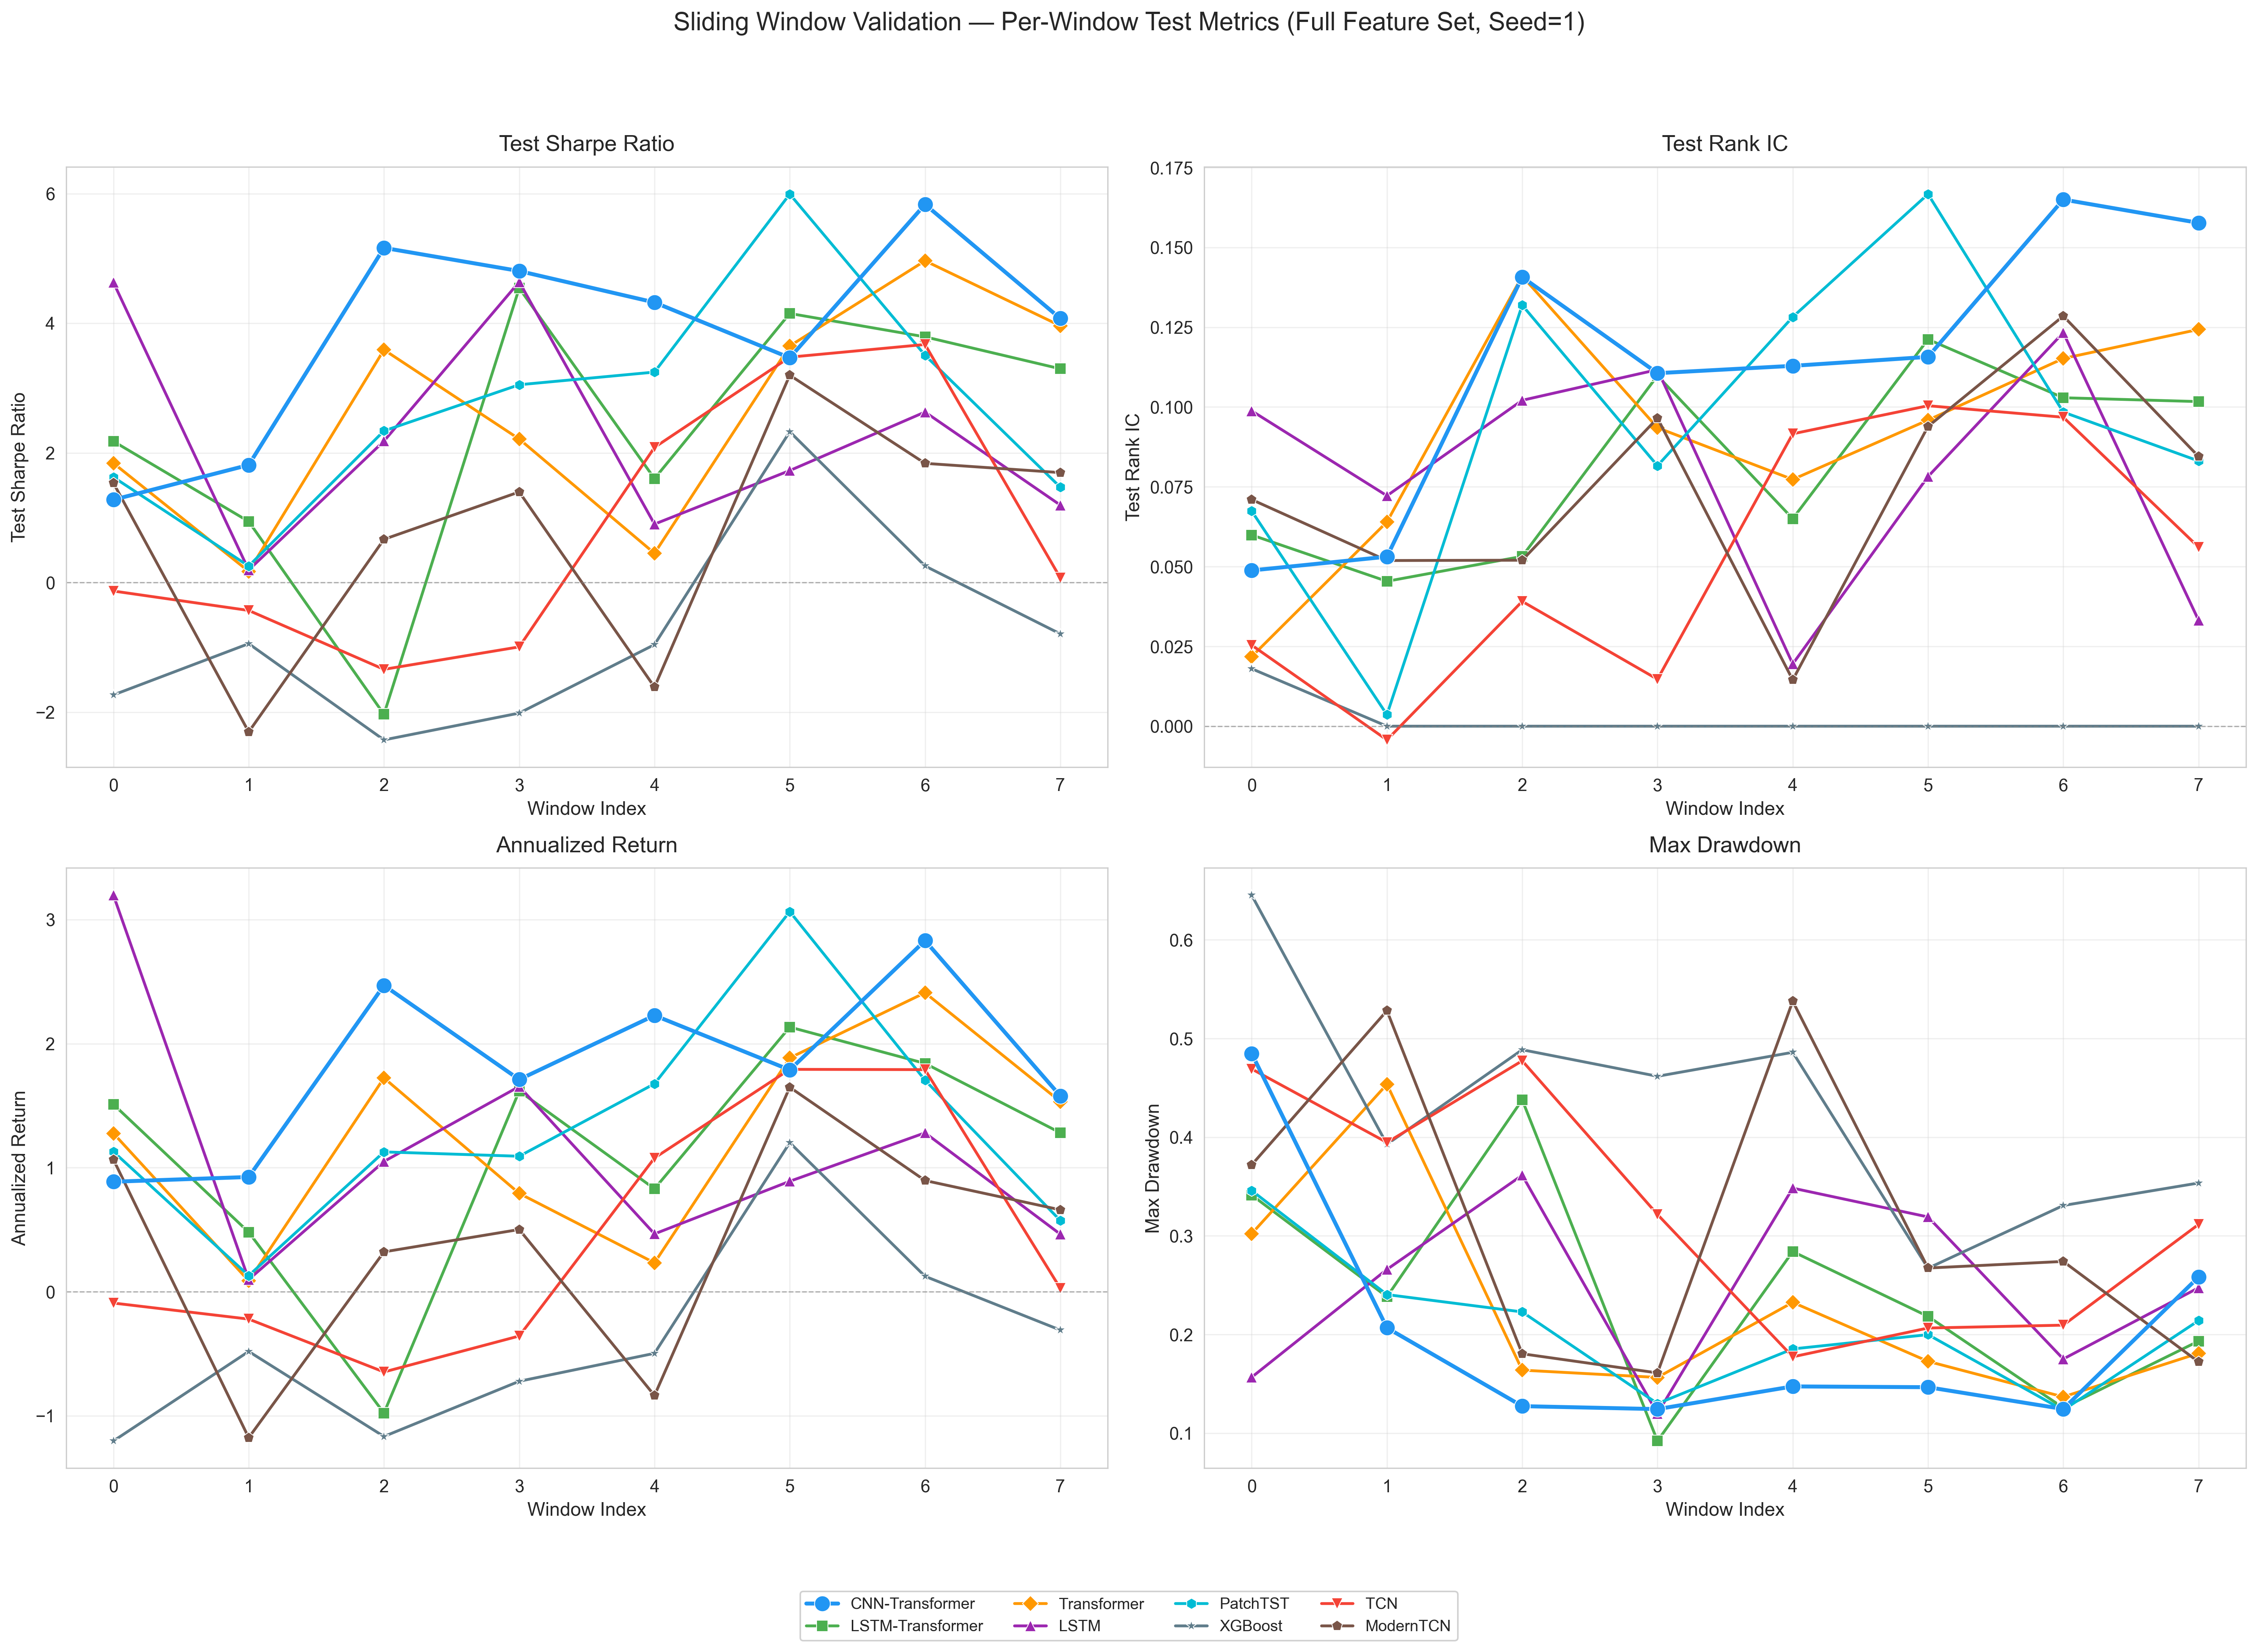
\includegraphics[width=0.95\textwidth]{../charts/sliding_window_metrics.png}
\caption{Sliding window validation: test Sharpe, IC, annual return, and maximum drawdown across windows on the full feature set (seed=1). Windows 0--7 sequentially cover 2022 H1 through 2025 H2, spanning bear, rebound, bull, and consolidation market regimes.}
\label{fig:sliding_window_metrics}
\end{figure*}

Table~\ref{tab:sliding_window} and Figure~\ref{fig:sliding_window_metrics} present the test performance of all 10 models across 8 time windows, with the following main findings:

(1) CNN-Transformer achieves the best sliding-window performance, with TimeMixer a strong second. CNN-Transformer achieves the highest cross-window mean (3.85, std 1.59) with a minimum of 1.28 (W0) and maximum of 5.83 (W6). TimeMixer ranks second with a cross-window mean of 3.19 (std 1.51), demonstrating that its multi-scale mixing architecture, despite its inability to exploit on-chain data (Section~6.2), maintains robust predictive power in dynamic market regimes. Four of ten models maintain positive Sharpe across all eight windows (CNN-Transformer, PatchTST, Transformer, LSTM), with TimeMixer and LSTM-Transformer positive in seven of eight windows (only W1=$-$0.01 and W2=$-$2.03, respectively).

(2) Sliding windows reveal a richer hierarchy than static evaluation. Cross-window means: CNN-Transformer (3.85) $>$ TimeMixer (3.19) $\gg$ PatchTST (2.69) $\approx$ Transformer (2.61) $\approx$ LSTM-Transformer (2.31) $\approx$ LSTM (2.26) $\gg$ ModernTCN (0.80) $\approx$ TCN (0.80) $\gg$ XGBoost ($-0.79$) $\approx$ DLinear ($-1.26$). XGBoost's static Sharpe (4.50) collapses under sliding windows, while DLinear's mean of $-1.26$ (std 2.15) confirms the linear model's structural inadequacy across all regimes.

(3) ModernTCN and TCN exhibit severe cross-window overfitting. ModernTCN's training Sharpe exceeds 32 in all 8 windows, yet its test-set mean is merely 0.80. DLinear shows extreme cross-window instability (std 2.15), oscillating between positive returns in some windows (+0.80 in W6) and catastrophic losses in others ($-5.38$ in W1). The on-chain synergy effect exhibits a ``market regime floor condition''---when derivative and sentiment signals weaken in bear markets, the incremental value of on-chain data is compressed.

\subsection{Discussion}

We discuss the results from four perspectives:

\begin{enumerate}[label=(\arabic*),leftmargin=1.5em]
    \item \textbf{Mechanistic interpretation of the conditional effectiveness of on-chain data.} SOPR and CDD reflect realized on-chain behavior and are inherently ``slow variables'' requiring ``activation'' through derivatives dynamics and market sentiment. An isolated SOPR below 1 is ambiguous; coinciding with extreme fear (FNG $<$ 25) and negative funding rate, the three-signal confluence substantially raises the probability of a panic bottom. Hybrid architectures' hierarchical pipeline (CNN local extraction $\to$ Transformer global interaction) is naturally suited to capturing such multi-source joint distributions: convolutional layers compress temporal patterns within local receptive fields, while self-attention models high-order cross-feature interactions across time steps. This mechanism explains the existence of the three-group taxonomy---pure recurrent/convolutional architectures lack global cross-feature interaction capability and miss cross-source synergistic signals; the PDM module in multi-scale mixing architectures (TimeMixer) processes each scale independently after decomposition, potentially disrupting the joint distribution structure of cross-source features.

    \item \textbf{Cautious interpretation of absolute performance levels.} The best model's cross-seed mean Sharpe of 5.19 and annualized return of 211.5\% should be regarded as upper-bound estimates: (1) the strategy omits margin and position constraints; (2) only 5 bps cost is deducted, whereas real-world costs reach 20--50 bps; (3) the period spans a BTC bull cycle; (4) annualization ($\times 2190$) amplifies single-period advantages. The relative ranking and cross-architecture consistency of the synergy effect are the transferable core conclusions. Future studies are advised to adopt the cross-window mean Sharpe under multi-seed sliding windows (e.g., 3.85 for the synergistic-utilization group) as a more conservative performance benchmark.

    \item \textbf{Transaction costs and turnover: from prediction to deployment.} Figure~\ref{fig:cost_sensitivity} shows cost sensitivity across 0--50 bps for six representative models; detailed values are reported in Table~\ref{tab:cost_sensitivity}.

    \begin{figure*}[t]
    \centering
    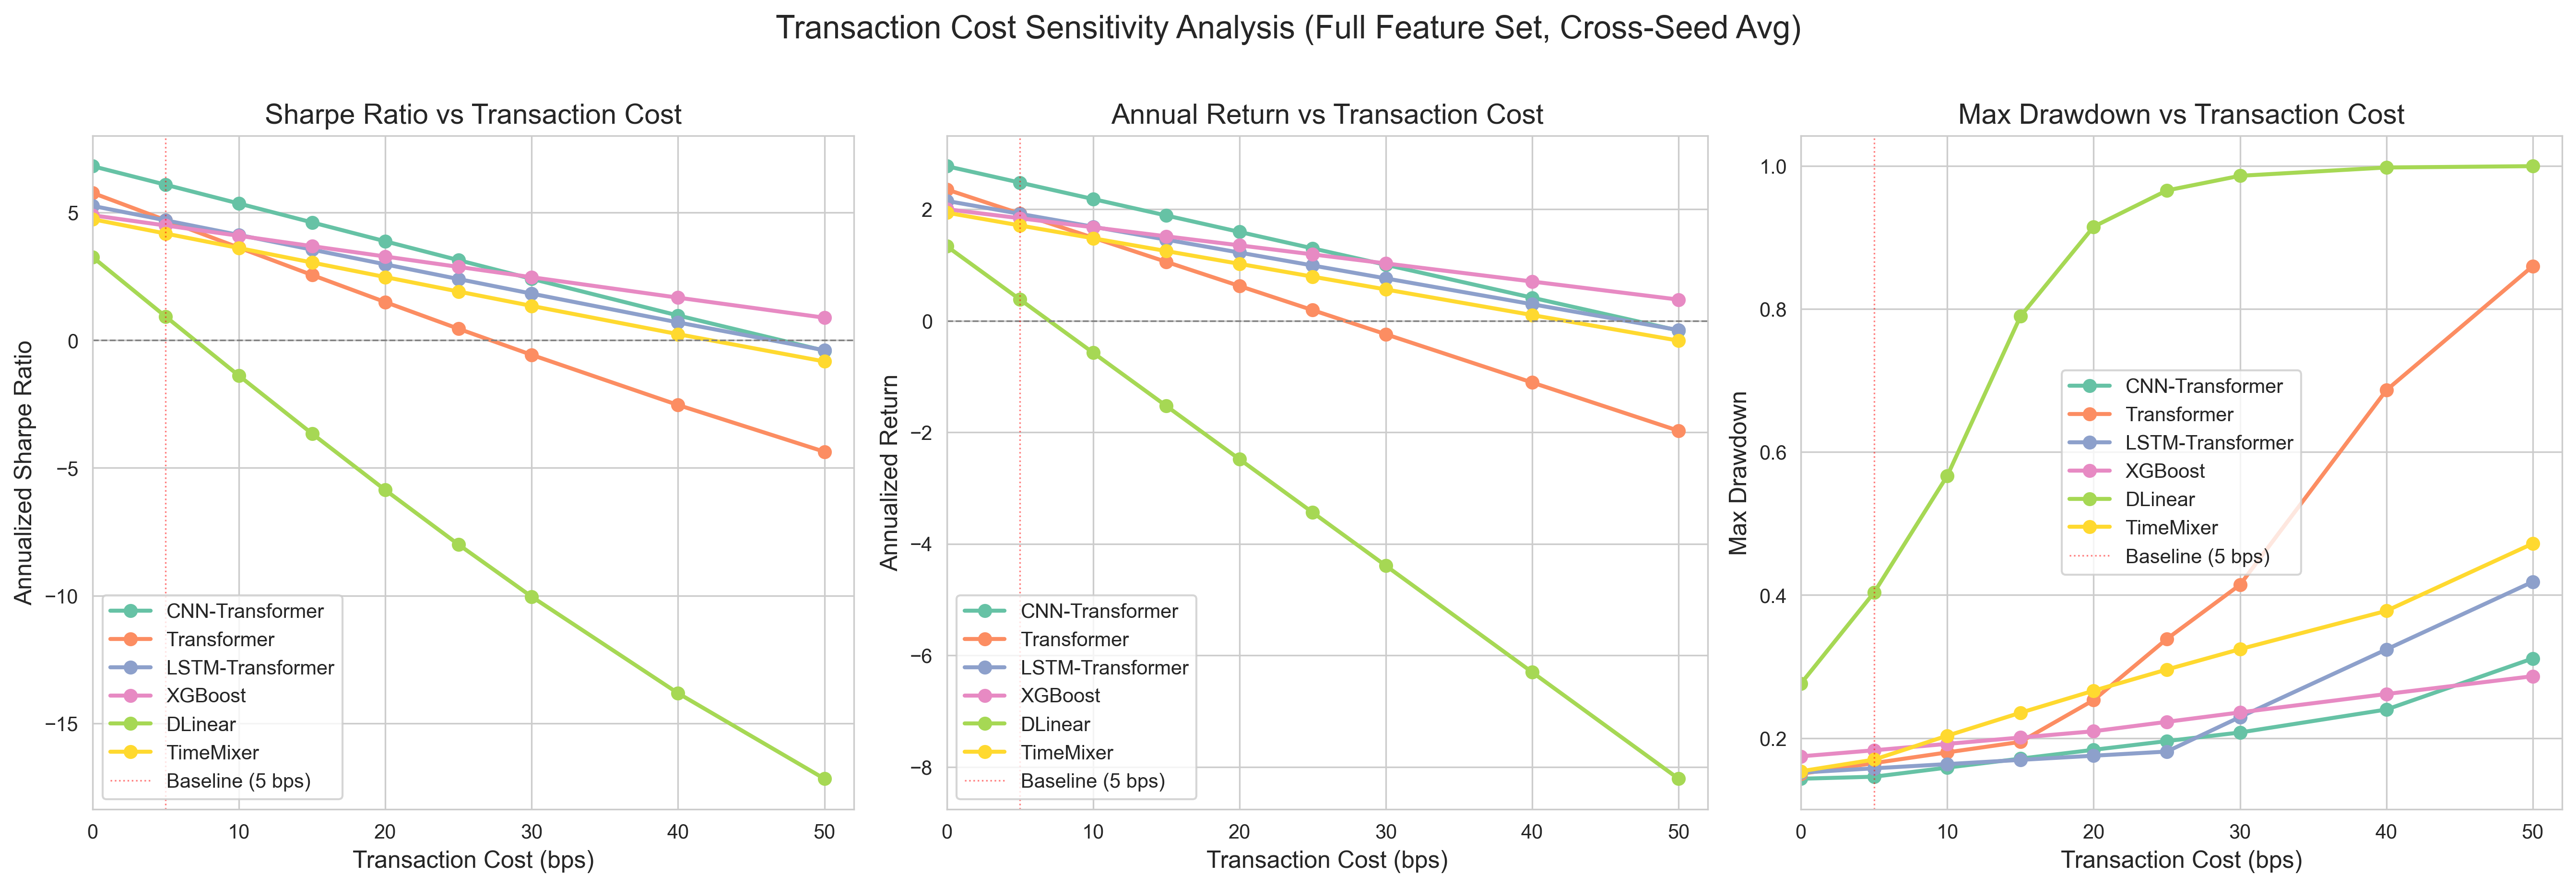
\includegraphics[width=0.95\textwidth]{../charts/cost_sensitivity.png}
    \caption{Transaction cost sensitivity analysis (full feature set, cross-5-seed mean): from left to right, the decay curves of Sharpe ratio, annual return, and maximum drawdown as transaction fees increase from 0 to 50 bps.}
    \label{fig:cost_sensitivity}
    \end{figure*}

    \input{../results/cost_sensitivity_en.tex}

    Break-even fees (Table~\ref{tab:cost_sensitivity}): hybrid architectures (CNN-Transformer 47 bps, LSTM-Transformer 46 bps) substantially outperform the pure Transformer (27 bps); at 20 bps their Sharpe decay (36--37\%) is far lower than the Transformer's 68\%. TimeMixer shows surprisingly robust cost resilience (break-even $\sim$42 bps) despite its inability to exploit on-chain data---its moderate turnover (11.0\%) limits transaction-cost erosion. At the opposite extreme, DLinear's break-even is merely $\sim$7 bps, driven by an unsustainable 46.0\% turnover rate (flipping positions approximately every 9 hours). Turnover data (Table~\ref{tab:turnover}) reveals the behavioral root of cost resilience: the CNN-Transformer's 17.9\% turnover lies in the medium-frequency sweet spot, while pure convolutional architectures reach 26--27\% and DLinear churns at 46.0\%. TimeMixer and LSTM-Transformer achieve the lowest turnover (11.0\% and 7.9\%) among deep models, consistent with their more conservative signal generation.

    % Auto-generated turnover rate LaTeX table (English)
\begin{table*}[t]
\centering
\caption{Turnover rate and holding period comparison across models (full feature set, cross-seed average)}
\label{tab:turnover}
\footnotesize
\setlength{\tabcolsep}{5pt}
\resizebox{\textwidth}{!}{%
\begin{tabular}{lcccc}
\toprule
Model & Turnover (\%) & Annual Turn. & Hold (hours) & Hold (days) \\
\midrule
XGBoost & 6.7 & 146 & 60 & 2.5 \\
LSTM-Transformer & 7.9 & 173 & 51 & 2.1 \\
TimeMixer & 11.0 & 241 & 36 & 1.5 \\
LSTM & 12.1 & 264 & 34 & 1.4 \\
CNN-Transformer & 17.9 & 392 & 23 & 0.9 \\
Transformer & 22.8 & 499 & 18 & 0.7 \\
TCN & 26.7 & 585 & 15 & 0.6 \\
ModernTCN & 26.8 & 587 & 16 & 0.6 \\
PatchTST & 27.0 & 591 & 15 & 0.6 \\
DLinear & 46.0 & 1006 & 9 & 0.4 \\
\bottomrule
\multicolumn{5}{l}{\footnotesize Turnover = fraction of time steps with position sign change. Annual turnover = turnover $\times$ 2190. Cross-5-seed mean.} \\
\end{tabular}%
}
\end{table*}


    \item \textbf{Practical implications for architecture selection.} The three-group taxonomy provides clear guidance for real-world deployment. When on-chain features are available, hybrid architectures (CNN-Transformer, LSTM-Transformer) should be preferred to unlock cross-source synergy, and they also offer superior cost resilience (break-even $\sim$47 bps). When on-chain data cannot be incorporated due to acquisition costs or inference-latency constraints, multi-scale mixing architectures such as TimeMixer achieve the best performance on price+funding+sentiment feature sets (Sharpe 4.89) with surprisingly robust cost resilience (break-even $\sim$42 bps). Pure attention architectures (Transformer, PatchTST) are a safe default when feature-set composition is uncertain, as they are neutral to on-chain addition. Pure recurrent and pure convolutional architectures systematically deteriorate with on-chain features and should be avoided in multi-source heterogeneous settings. Notably, XGBoost's collapse under sliding windows (static Sharpe 4.50 $\to$ mean $-0.79$) serves as a cautionary note: a tree model's high static Sharpe may constitute ``lucky overfitting,'' and sliding-window-based temporal cross-validation should become standard practice in financial forecasting model evaluation. DLinear's near-zero cross-window mean ($-1.26$) further confirms that purely linear decomposition methods have limited utility in highly nonlinear multi-source heterogeneous settings.
\end{enumerate}

\section{Conclusion and Outlook}

This paper makes three principal contributions to multi-source heterogeneous data fusion for financial forecasting, demonstrated through a systematic case study of on-chain indicators for cryptocurrency returns:

\begin{enumerate}[label=(\arabic*),leftmargin=1.5em]
    \item The conditional-effectiveness principle. We demonstrate that the predictive value of on-chain data is conditional, not universal: short-term on-chain indicators (SOPR/CDD) are detrimental in isolation yet produce a large, statistically significant Sharpe gain when combined with derivative and sentiment features---provided the architecture can exploit cross-source interactions. Long-term on-chain indicators show no predictive value at the 4-hour frequency.
    \item The three-group architecture taxonomy. We discover that on-chain synergy exhibits a clear architecture-dependent pattern: the ten tested models separate into a synergistic-utilization group (CNN-Transformer, LSTM-Transformer; $\Delta$Sharpe $> +2$), a neutral group (Transformer, PatchTST, DLinear, XGBoost; $\Delta$Sharpe $\approx 0$), and a negative-interference group (LSTM, TCN, ModernTCN, TimeMixer; $\Delta$Sharpe $< -1.5$). This taxonomy is consistent across five random seeds and robust under sliding-window validation. The core insight is the feature set $\times$ model architecture interaction effect rather than any single model's absolute ranking.
    \item From prediction to deployment: cost resilience and temporal robustness. We establish a multi-dimensional evaluation chain and find that hybrid architectures exhibit approximately double the cost resilience of pure architectures (break-even $\sim$47 bps vs.\ $\sim$27 bps), behaviorally rooted in moderate turnover rates. The three-group pattern persists across eight market regimes (2022--2025), with the synergistic-utilization group achieving the highest cross-window mean Sharpe (3.85). TimeMixer ranks second (mean 3.19), demonstrating that architectures which fail to exploit on-chain synergy can nonetheless maintain competitive performance through multi-scale temporal mixing. At the other extreme, DLinear's cross-window mean of $-1.26$ confirms the inadequacy of purely linear decomposition. XGBoost's high static Sharpe (4.50) collapses under sliding windows (mean $-0.79$)---a methodological caution that single-window evaluation can severely mislead model selection in financial forecasting.
\end{enumerate}

Limitations include: (1) the study only spans BTC; cross-asset validation is needed---Ethereum and other smart-contract platforms feature on-chain data with fundamentally different economic semantics (e.g., gas consumption, DeFi total value locked), and whether their on-chain data follows a similar conditional-dependence mechanism to BTC remains unknown; for traditional assets (equities, FX) that lack on-chain data entirely, whether the methodological framework can be partially adapted (e.g., substituting on-chain variables with capital-flow or order-flow indicators) merits exploration; (2) the conclusions are conditional on the 4-hour frequency; the effectiveness of on-chain data may shift qualitatively across time scales---at daily or weekly horizons, long-term on-chain indicators (exchange balances, active addresses) may gain predictive power as their fluctuation cycles better match macro supply-demand rhythms; at 1-hour or minute-level frequencies, market-microstructure noise may overwhelm on-chain signals, and the stability of both the ``conditional effectiveness'' thesis and the three-group architecture taxonomy across temporal granularities requires further validation; (3) cross-source interaction relies on hand-crafted terms; graph neural networks may offer a more systematic framework; (4) more realistic trading simulation (incorporating margin constraints, position limits, and slippage) could be explored; (5) sliding window validation uses a single seed and could be extended to multiple seeds.

\acknowledgment{This work was supported by the Humanities and Social Sciences Project of the Ministry of Education of China (Grant No.\ 19YJCZH031) and the Shanghai Municipal Education Science Research Project (Grant No.\ C2023068).}

\declaration[Declaration of Competing Interest]{The author declares that he has no known competing financial interests or personal relationships that could have appeared to influence the work reported in this paper.}

\printcredits

%% ---- Bibliography ----
\bibliographystyle{cas-model2-names}
\bibliography{cas-refs}

%% ---- Author Biography ----
\bio{}
Minghan He is currently a student at the School of Computer and Information Engineering, Shanghai Polytechnic University. His research interests include deep learning, financial time series forecasting, and quantitative finance.
\endbio

\end{document}
